\documentclass{article}
\usepackage[utf8]{inputenc}
\usepackage{subfigure}
\usepackage{geometry}
\usepackage{amsmath}
\usepackage{graphicx}
\usepackage{pgfplots}
\usepackage{pgfplotstable}
\graphicspath{ {./images/} }
\title{Silver Crest/Stem Biology}
\author{Sirius Chan}
\begin{document}
\maketitle

\newpage

\section{Investigation aim}

The STEM biology class was introduced to culturing fruit flies last year. I noticed that flies in many of the vials did not survive because of various reasons, usually because they were stuck to the side of the vial or because the media mix (food) dried out. This led me to wonder how well fruit flies react to different environments.

\noindent\\
The investigation aims to figure out "how variations in the environment affect the survival and reproduction of fruit flies", more specifically, what will happen if they experience a serious shortage in glucose and protein sources.

\subsection{Hypothesis}

The hypothesis is that when there are not enough nutrients, the fruit flies would prioritise reproduction over their survival. This could be a result of evolution because, without reproduction, all fruit flies would die out. Given that they are not extinct, therefore they should be naturally hardwired to prioritise reproduction.

\noindent\\
Another part of the hypothesis is that because glucose provides the fruit flies energy for daily activity, and protein is responsible for growth-related functions, fruit flies with insufficient glucose only will survive but be unable to reproduce, and those with insufficient protein only will be able to reproduce but not to survive.

\subsection{How the hypothesis can be evaluated}

\subsubsection{"Reproduction over survival" hypothesis}
The requirements for verifying the first hypothesis are:

\begin{itemize}
    \item When there is sufficient glucose and protein, both the reproduction rate and survival rate should be "high".
    \item When the amount of glucose and yeast decreases to an insufficient level, we should see a more significant drop in survival rate while the reproduction rate remains relatively high; this is because, according to the hypothesis, they will prioritise reproduction over survival.
    \item Many larvae (baby fruit flies) will not grow up into adult fruit flies when there are insufficient nutrients because while there is a relatively large number of eggs laid, only a tiny fraction of them will survive to become adults.
\end{itemize}

\noindent
There should be a clear point between "sufficient" and "insufficient" glucose and protein. This point might look something like a sharp turn on the results graph - to the right both reproduction and survival rate plateaus as something else is the limiting factor (such as how quickly can eggs be produced for reproduction, the age for survival), and to the left reproduction and survival rates declines relatively quickly as the malnourishment becomes the limiting factor.

\noindent\\
If the hypothesis is correct, the survival rate should decline quicker than the reproduction rate past the "point of malnourishment".

\subsubsection{"Different roles of glucose and protein" hypothesis}

\noindent
The requirements for verifying the second hypothesis are:

\begin{itemize}
    \item As the concentration of glucose drops, there should be fewer surviving adult fruit flies. As glucose is required for survival.
    \item As the concentration of protein drops, there should be fewer eggs/larvae/pupa (cocoon-like thing), as they are produced in the process of reproduction and growth.
    \item A decrease in protein should not have an as great impact on the number of surviving fruit flies as glucose, as glucose is responsible for living whereas protein is not so much so.
    \item A decrease in glucose should not inhibit growth or reproduction rate (larvae per adult fly), as the roles of glucose do not extend to reproduction. This should be the same as vice versa if the hypothesis is correct.
\end{itemize}

\noindent\\
If the hypothesis is correct, taken to the two extremes, things should happen are:

\begin{itemize}
    \item When there is no glucose but sufficient protein, there should be much presence of larvae and pupa, while lacking any alive adult fruit flies.
    \item When there is no protein but sufficient glucose, the initial fruit flies will live a long time before they die, but with no reproduction.
\end{itemize}

\subsection{Issues with the hypotheses}

Most of the issues with the hypotheses are not realised until halfway through the experiment when they give unexpected or difficult-to-interpret results.

\begin{enumerate}
    \item It is very vague to evaluate if the hypothesis stands based on "if the reproduction rate does not decline as quickly as survival rate" - first of all, the baseline for the normal rate of survival and reproduction is not determined. But there is nothing called a "normal rate", the more sufficient the nutrients are, of course, they will survive better and reproduce more.
    \item It was assumed that glucose and protein have very distinct roles to fruit flies, only responsible for their survival rate and reproduction/growth respectively and not the other. However, during the experiment, most of the flies with insufficient glucose supply seemed to be surviving just fine. This can be caused by the fact that protein can also be used as a source of energy, and to a degree replace the role of glucose. This is not realised until halfway through the experiment and made evaluating the 2nd hypothesis a lot more difficult.
\end{enumerate}

\newpage
\section{Investigation methodology}

To test the hypotheses, it will be necessary to place fruit flies in various environments with different levels of glucose and protein availability. This can be done by putting the fruit flies into different vials, each vial containing an agar gel substance, plus a different amount of sucrose (for glucose) and dried brewers yeast (for protein).

\subsection{Composition}

I asked Dr. Bass for the formula of the fruit fly media (food) mix because he showed us in the STEM biology class how to keep fruit flies.

\noindent\\
The formula for the media mix is:\\

{
\centering
\begin{tabular}{|c|c|}
  \hline
  Item & Amount\\
  \hline
  \hline
  Distilled water & 500ml\\
  Agar & 5g\\
  Brewers yeast & 50g\\
  Sucrose & 50g\\
  Propionic acid & 2ml\\
  Methyl 4-hydroxybenzoate & 0.5g\\
  Ethanol & 1.3ml\\
  \hline
\end{tabular}
\par
}

\noindent\\\\
Where propionic acid and methyl-4-hydroxybenzoate (dissolved in ethanol) are used as preservants so that the media mix doesn't mould.

\subsubsection{Variables}

In the experiment, each vial will be made of slightly different concentrations of sucrose and yeast. Below are the sucrose and yeast concentrations of the different vials:\\


{
\centering
\begin{tabular}{|c|c|c|}
  \hline
  Vial & Sucrose ($g/dm^3$) & Yeast ($g/dm^3$)\\
  \hline
  \hline
  1 & 75 & 75\\
  2 & 67.5 & 67.5\\
  3 & 60 & 60\\
  4 & 52.5 & 52.5\\
  5 & 45 & 45\\
  6 & 37.5 & 37.5\\
  7 & 30 & 30\\
  8 & 22.5 & 22.5\\
  9 & 15 & 15\\
  10 & 0 & 0\\
  \hline
\end{tabular}
\begin{tabular}{|c|c|c|}
  \hline
  Vial & Sucrose ($g/dm^3$) & Yeast ($g/dm^3$)\\
  \hline
  \hline
  11 & 60 & 75\\
  12 & 45 & 75\\
  13 & 30 & 75\\
  14 & 15 & 75\\
  15 & 0 & 75\\
  \hline
  16 & 75 & 60\\
  17 & 75 & 45\\
  18 & 75 & 30\\
  19 & 75 & 15\\
  20 & 75 & 0\\
  \hline
\end{tabular}
\par
}
\noindent\\
These vials will be referred to in a format of S/Y, where S is the concentration of sucrose and Y is the concentration of yeast. For example, vial no. 1 will be 75/75 and vial 16 will be 75/60.

\noindent\\
Note that vials 7.5/7.5 is skipped to make a nice number of 20 vials.

\newpage
\noindent
The solutions needed are:

\begin{enumerate}
  \item 50$ml$ of 300$g/dm^3$ sucrose solution
  \item 50$ml$ of 300$g/dm^3$ brewer's yeast solution
  \item A 200$ml$ solution containing agar (powder), methyl 4-hydroxybenzoate (dissolved in ethanol) and propionic acid
\end{enumerate}

\subsubsection{Making the vials}

The materials needed are:\\

{
\centering
\begin{tabular}{|c|c|}
  \hline
  Item & Amount\\
  \hline
  \hline
  Distilled water & 300ml\\
  Agar & 3g\\
  Propionic acid & 1.2ml\\
  Methyl 4-hydroxybenzoate & 0.3g\\
  Ethanol & 1.3ml\\
  Brewers yeast & 15g\\
  Sucrose & 15g\\
  30ml vials & 20x\\
  \hline
\end{tabular}
\par
}

\noindent\\
Here's how the 20 vials of media can be made:

\begin{enumerate}
  \item Weigh out agar and place it in 1 litre Simax reagent bottle (a big glass bottle).
  \item Add 200ml of distilled water,  propionic acid and methyl 4-hydroxybenzoate (dissolved in 3ml of ethanol) to the bottle.
  \item In a separate (smaller) bottle, dissolve 15g of brewer's yeast (powder) in 50 ml of distilled water.
  \item In another separate bottle, repeat the same steps but with sucrose - dissolve 15g of sucrose in 50 ml of distilled water.
  \item Leave the 3 bottles cap loose and autoclave (sterialise by heating the bottles in hot water).
  \item Place all the bottles in a 55\textcelsius water bath to allow equilibration.
  \item Add an appropriate amount of sucrose and yeast solution into each vial - 10ml of a solution should give the vial 75$g/dm^3$ of that dissolved substance. For example, 37.5$g/dm^3$ can be made by adding only 5ml of that solution to the vial.
  \item Add extra distilled water to the vials where less sucrose or yeast solution is put in, this is to make sure that the volume of media in each vial is the same, it also dilutes the media to the desired concentration.
  \item Cap vials and store in a fridge, wait for them to set.
\end{enumerate}

\newpage

\subsubsection{Problems with this formula}


As the number of alive fruit flies may be moving all around, they need to be put unconscious before they are counted. When all the fruit flies are unconscious (and not moving), the number of active fruit flies can be calculated using the difference between the total number of flies and the number of flies inactive before putting them to sleep.

\subsubsection{Number of larvae}

larvae of fruit flies dig into the media mix and stay there before they turn into adults. As a result, only the larvae near the edge of the vial can be seen and counted, because the media mix is opaque and larvae in the middle cannot be seen.

\subsubsection{Number of pupa}

Pupa forms on the side of the vials when the larvae are ready to become adult flies, they are easy to count as they are clear visible shapes lined on the wall.

\subsubsection{Dead fruit flies}

Any fruit flies that don't move are considered dead, so it should be simple to figure out the dead numbers.

\subsection{Evaluating results}

The final phase of the investigation is to evaluate results and draw conclusions on whether the hypotheses were correct, this can be done in a few ways.

\subsubsection{First hypothesis}

The first hypothesis says that the decrease in survival rate should be higher than the reproduction rate when the flies are malnourished. So a reasonable prediction will be that, the reproduction rate to survival rate ratio will be higher for malnourished flies.

\begin{align*}
  \text{reproduction rate}&=\frac{\text{no. of larvae + pupa the week they appeared}}{\text{initial no. of flies}}\\
  \text{survival rate}&=\frac{\text{no. of adult flies after 2 weeks}}{\text{no. of larvae + pupa the week they appeared}}\\
  \text{reproduction-survival ratio}&=\frac{(\text{no. of larvae}+\text{pupa})^2}{\text{initial no.}\times\text{adult flies}}
\end{align*}

\noindent
The hypothesis can be supported by a graph where the line of best fit sloped up as the concentration of substances decreases.

\noindent\\
Data from the "main sequence" vials, where the concentration of yeast and sucrose are "one to one" (75/75 to 0/0) can be used. The 75/X and X/75 sequences of vials can also be used, but the differences in results may be caused by other factors than what is described in the hypothesis.

\subsubsection{Second hypothesis}

The second hypothesis predicts that the vial with no yeast will have no reproduction, whereas the vial with no sucrose will have reproduction but no surviving flies.

\noindent\\
By comparing the vial with 75$g/dm^3$ yeast and no sucrose, against the vial with no yeast but 75$g/dm^3$, there should be a clear difference that fits the prediction from the hypothesis. While this prediction also applies to vials with less contrasting concentrations (for example, a 75/45 vial against a 45/75 vial), they may not fit well in the prediction as their results are more likely to be affected by random factors such as if the flies are injured when being put into the vials.

\noindent\\
According to the hypothesis:

\begin{itemize}
  \item There should be more larvae/pupa when there is a higher concentration of yeast.
  \item These should be more surviving flies when there is a higher concentration of sucrose.
\end{itemize}

\noindent\\
After some research 1g of sucrose provide around 16kJ of energy, while protein from 1g of yeast only provides 2kJ of energy. Vials receiving less sucrose will not be able to completely replace it with the supply of yeast, so 0/75 (no sucrose) should not include sufficient energy for the flies.

\noindent\\
Plot two graphs, one graph containing the survival rate and reproduction rate of 75/X vials, and the other graph for X/75 vials. The 75/X graph should have a steeper slope for reproduction and a flatter slope for survival, the opposite should be true for X/75 vials.

\subsection{Factors affecting results}

Everything affects results, such as temperatures. But some things make the experiment unfair, as they may affect individual vials more.

\begin{enumerate}
  \item Number of flies - male/female: reproduction should be the most efficient when there is around an equal number of male and female flies (maybe more females, but it's too complicated), so it would be best if the number of male and female flies in each vial is the same. Random variations in the small number of flies in each vial can result in the experiment producing incoherent gibberish.
  \item Sunlight - it is shown in the experiment that the flies can realistically die from the media mix drying out. This is not known when planning the experiment, the rack of vials containing fruit flies was placed at a location near the window where each vial gets an uneven amount of sunshine. Although the position of the vials is shuffled every week (I put them back onto the rack randomly after each recording), unintentionally reducing the effects, it still results in some vials of media mix completely drying out with all flies inside dying. Or even worse, not all of them died and the vial continues to be recorded as valid data.
  \item Dead flies - some flies are dead before they are put in the vials for various reasons (will mention later), so it's important to note that although the recording says that all vials start with 9 flies, vials have around 1 dead fly on average and it is not recorded, or known how many flies the vials have initially.
\end{enumerate}

\newpage

\section{Practical}

The practical started on 23rd March, and the final experiment ended on 19th June.

I have:\\

\begin{itemize}
  \item All the materials I need to make the media mix
  \item 20 vials
  \item A big vials of flies (wild type adults)
  \item FlyNap
  \item Ice and water
\end{itemize}

\noindent\\
A total of 5 recordings were taken, each more than 1 week apart.

\subsection{Preparation}

The preparation was done before the Easter holidays so that the experiment can start after the holidays. Also, the flies haven't arrived yet so hopefully they will arrive after/during the holidays.

\subsubsection{Noon, 23rd March}

I was given 3 glass bottles and all the materials to make the three solutions for the media mix. Each substance is weighed and placed in the correct bottles respectively.

\noindent\\
They are then put to autoclave and left in a 55\textcelsius\space water bath.

\begin{figure}[ht]
  \centering
  \subfigure[Before preparation]{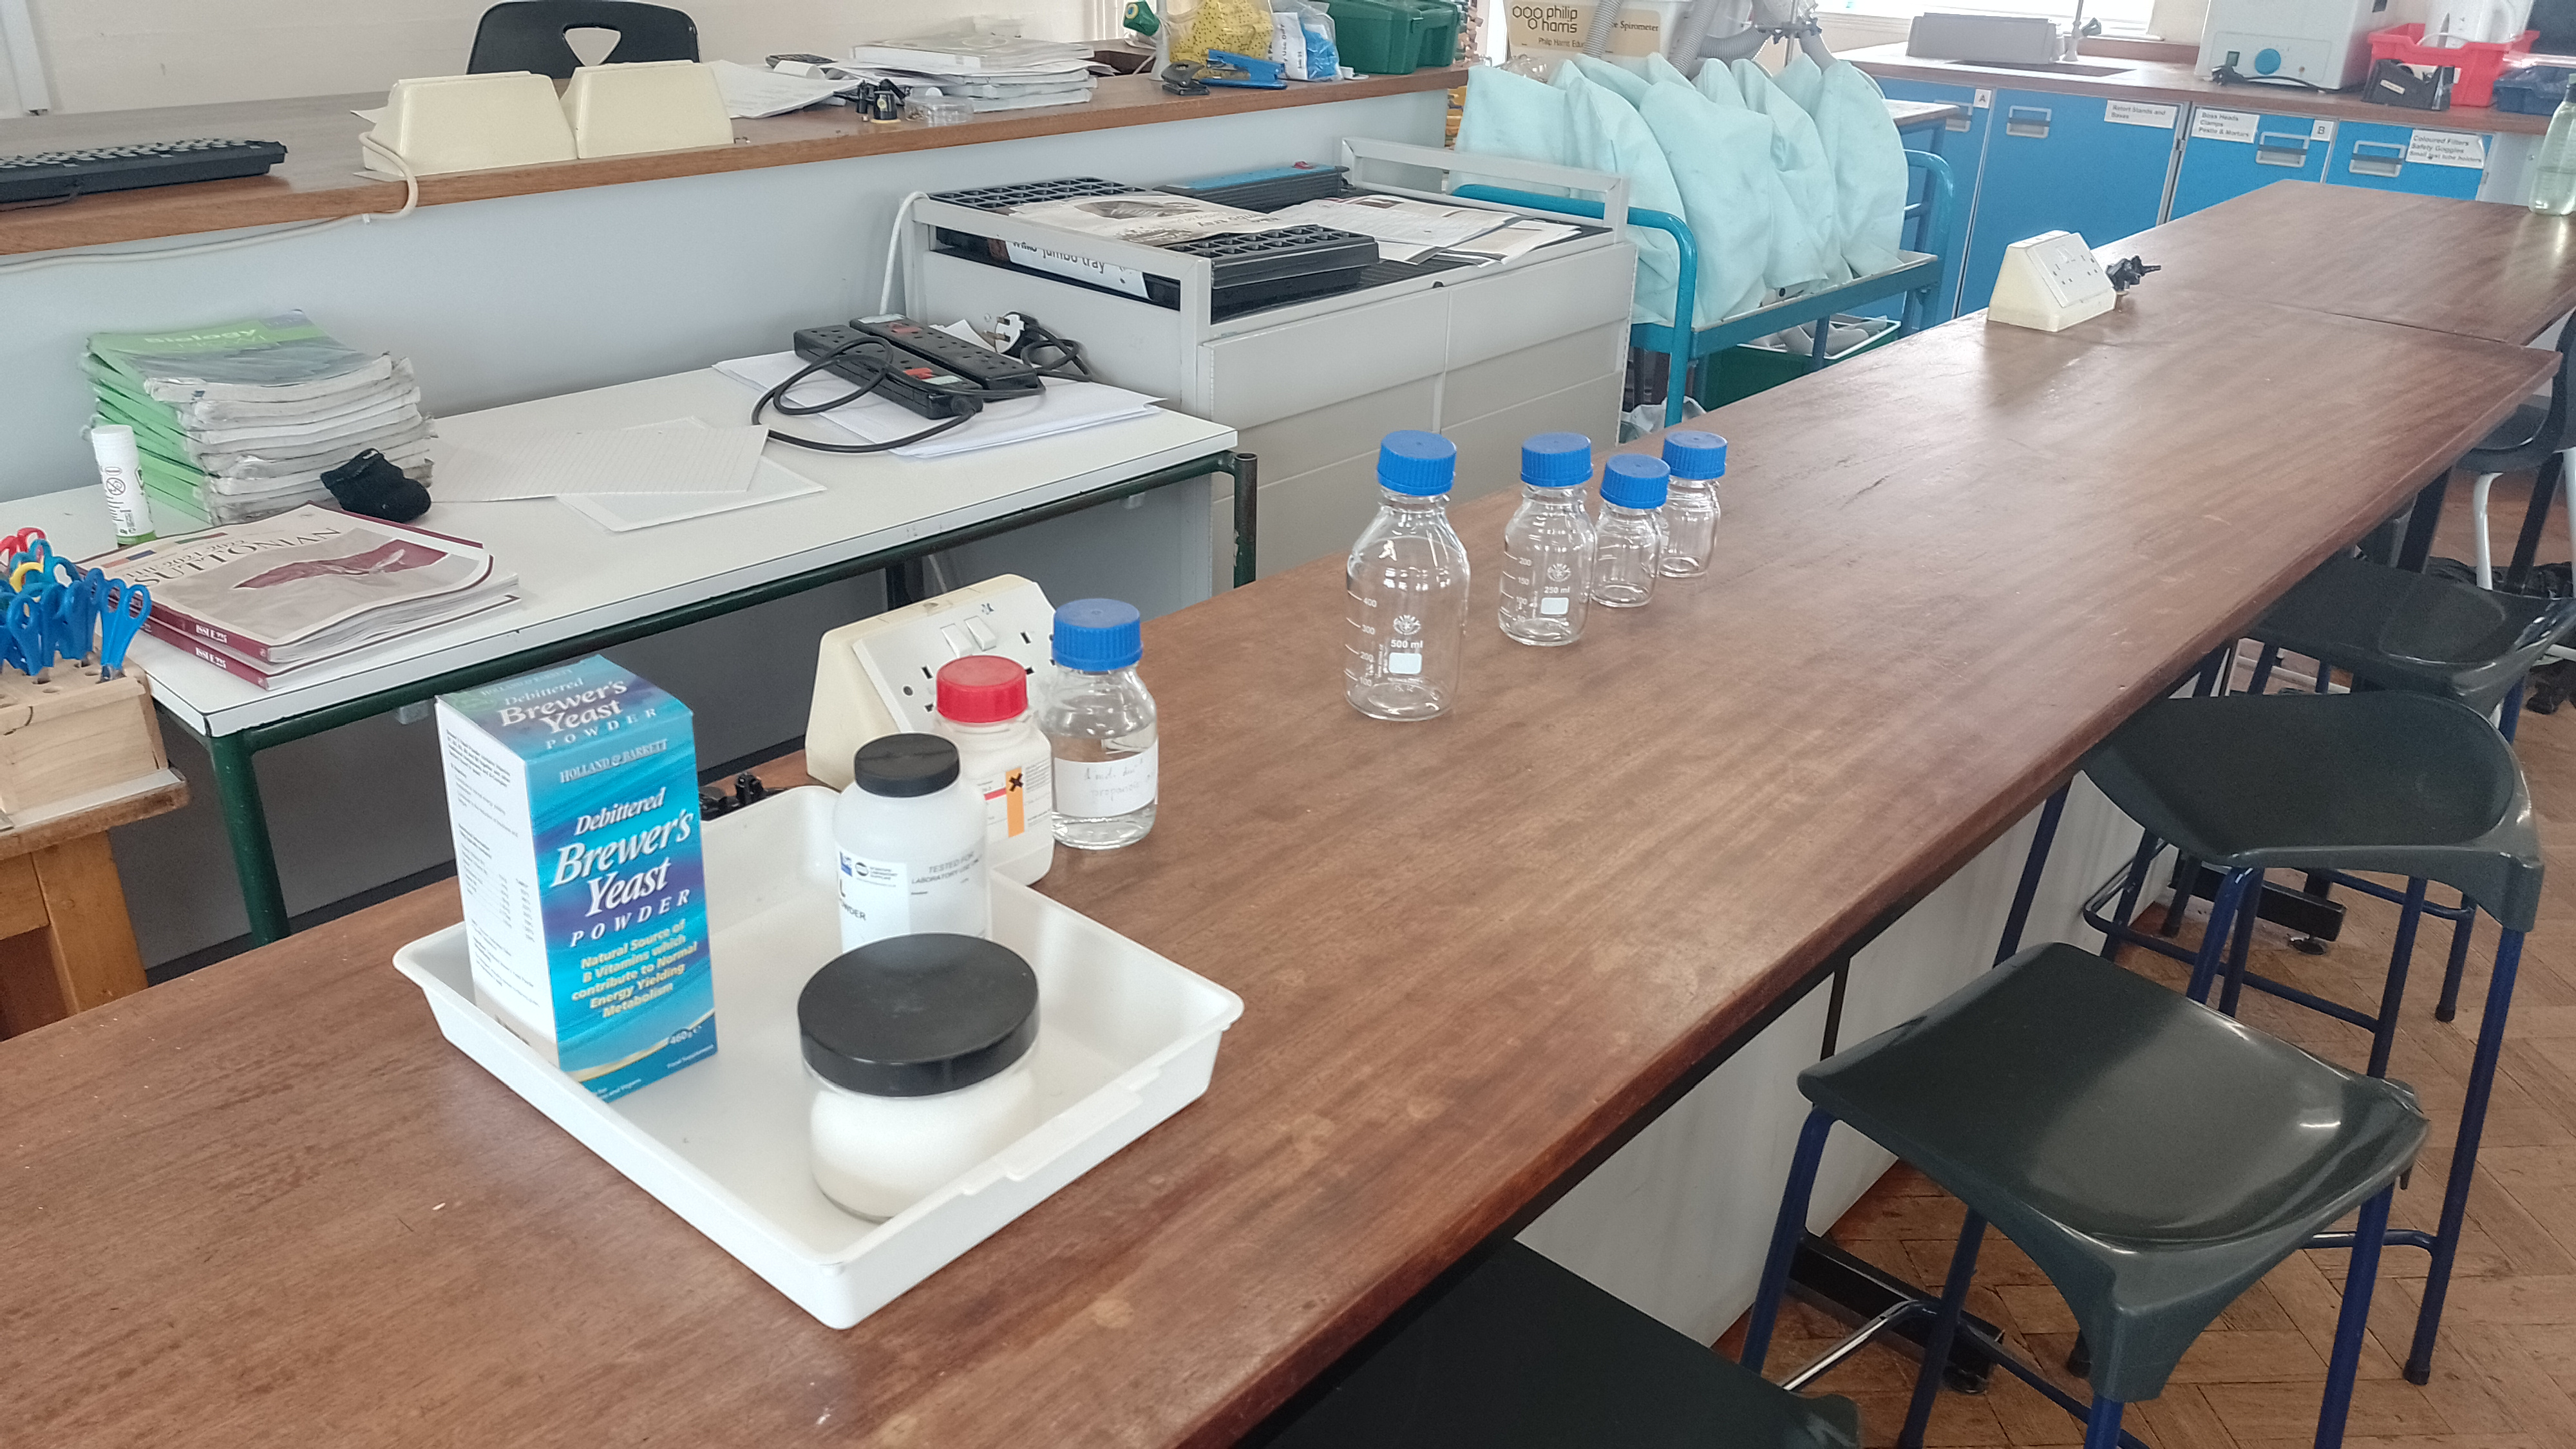
\includegraphics[width=0.45\textwidth]{prep-before}}
  \hfill
  \subfigure[Agar, sucrose and yeast solution prepared in separate bottles]{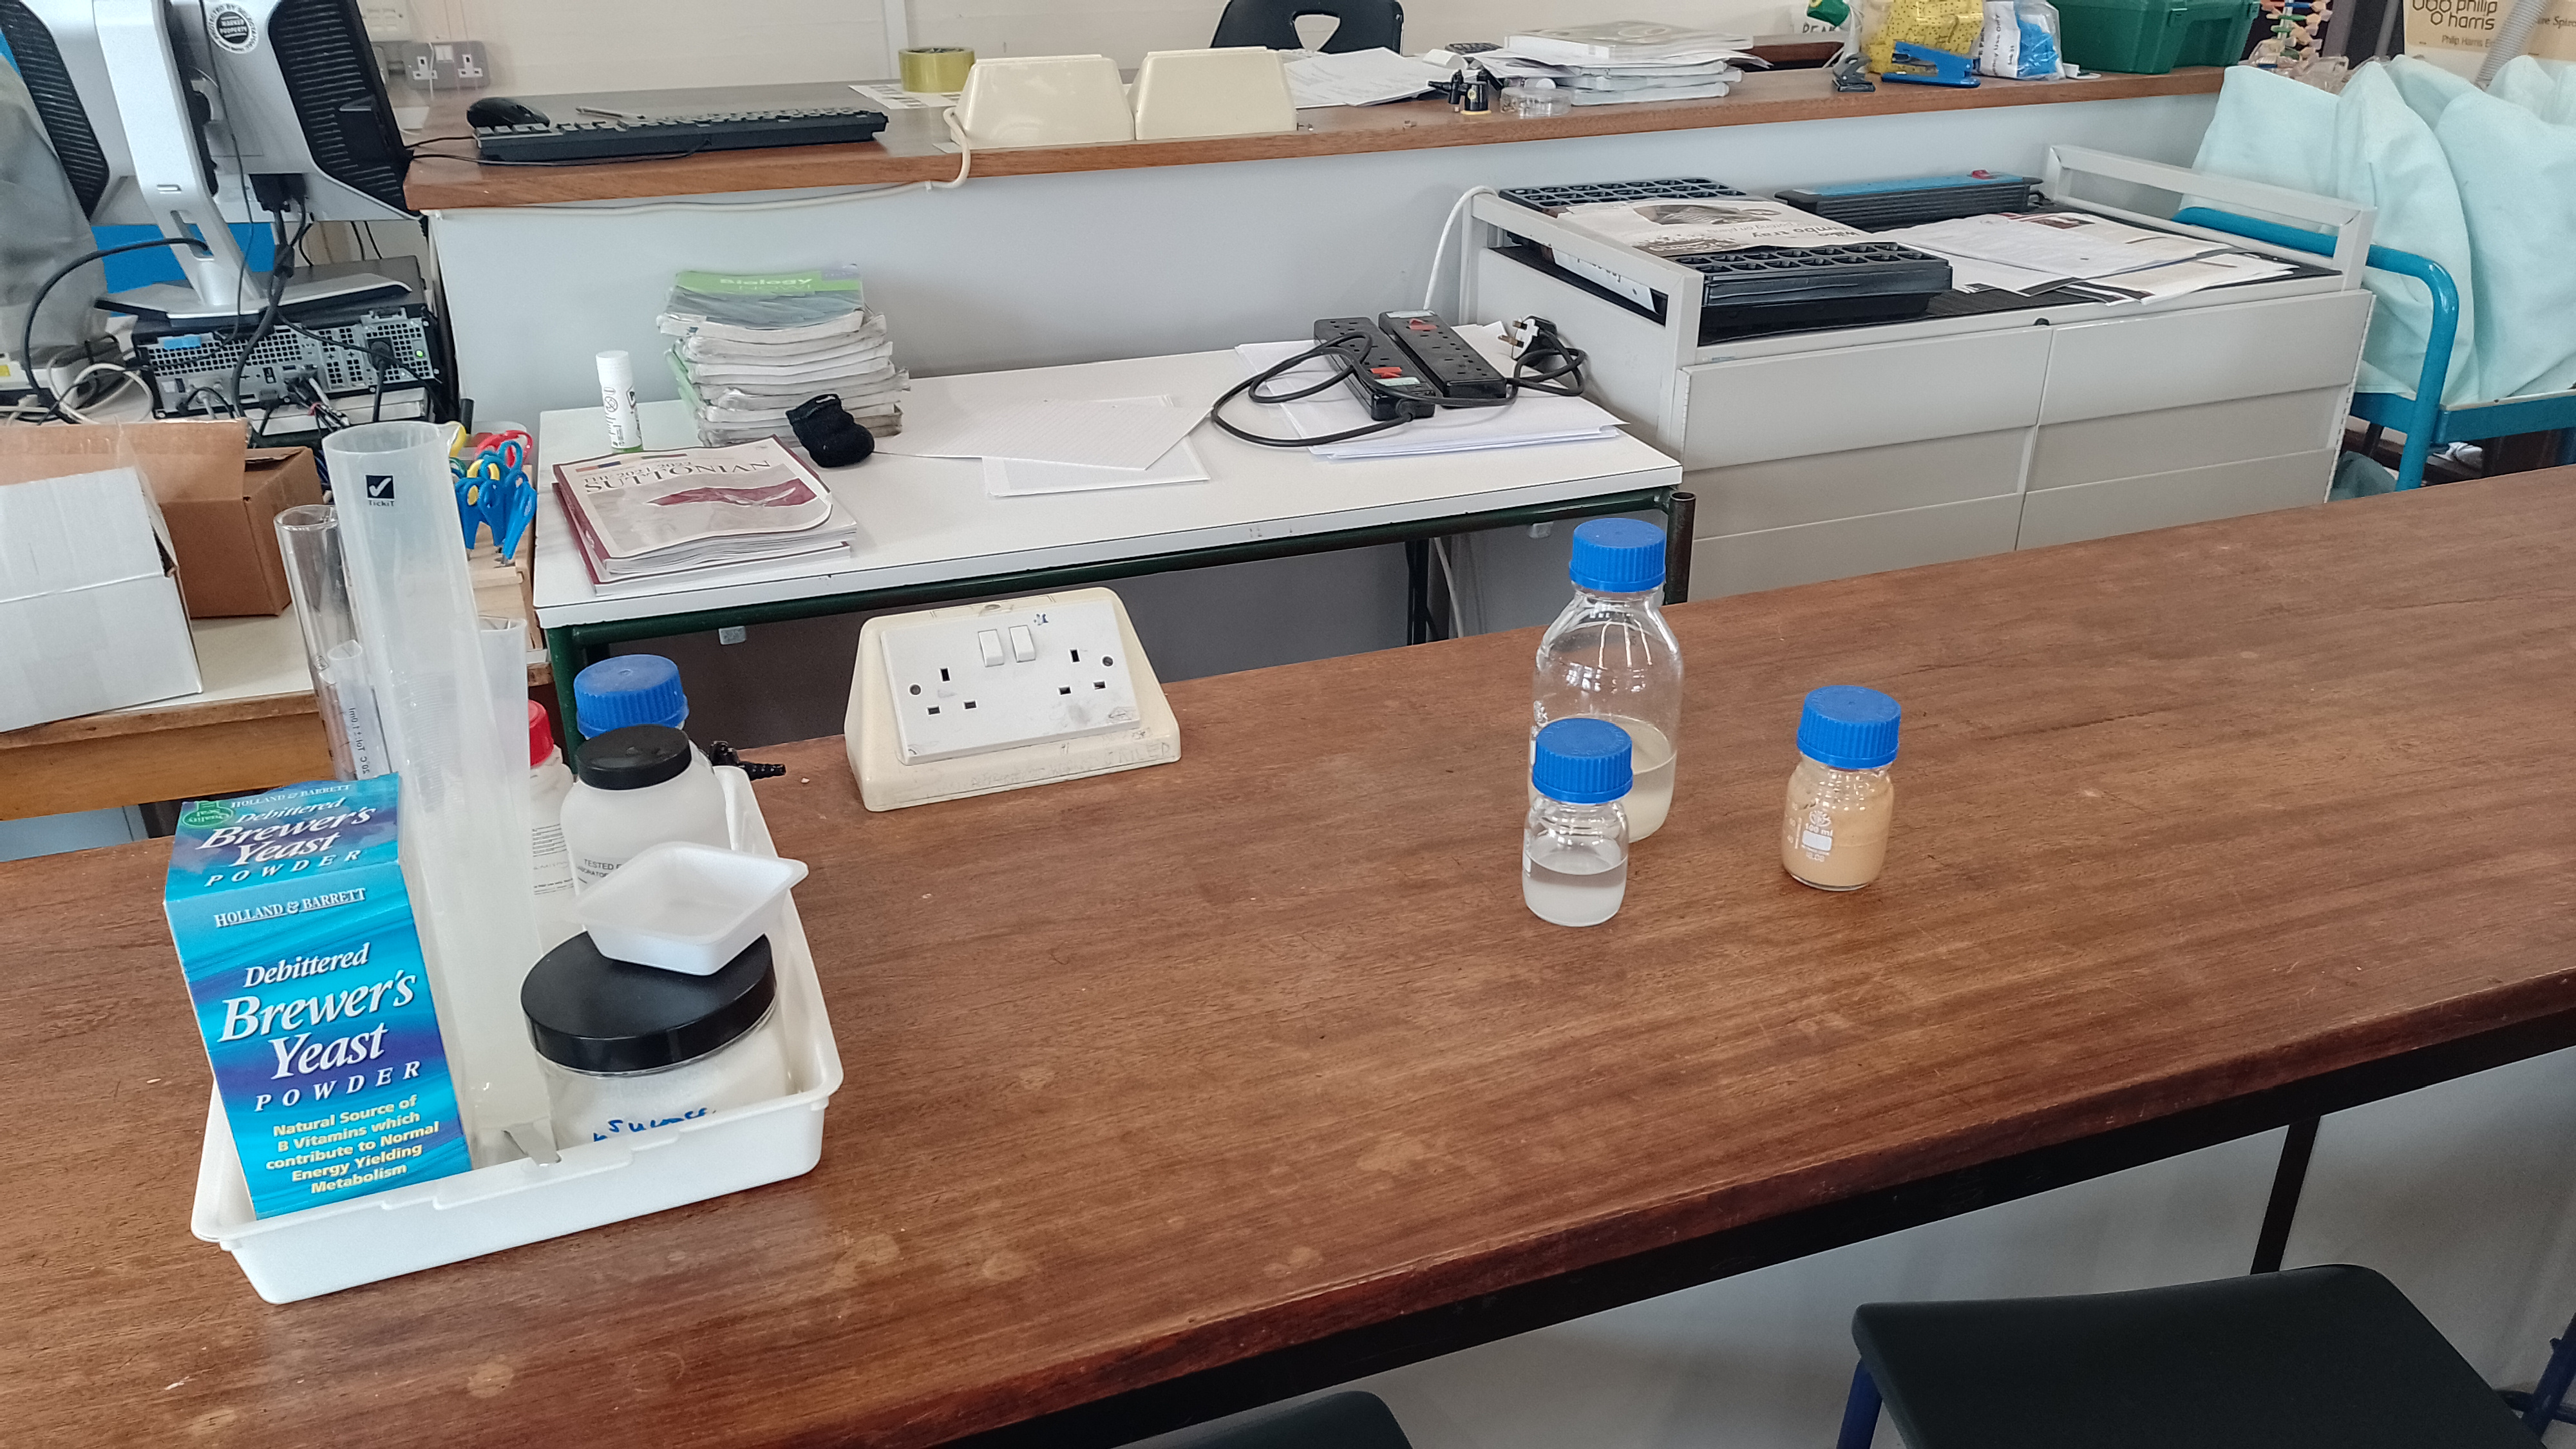
\includegraphics[width=0.45\textwidth]{prep-after}}
\end{figure}

\noindent
The vials are:

\begin{itemize}
  \item 200ml of agar solution (with more things mixed in)
  \item 50ml of concentrated sucrose and yeast solution respectively
\end{itemize}

\subsubsection{Afternoon, 23rd March}

With the 3 solutions in a water bath, they were added to the vials with a dropper, each vial got:

\begin{itemize}
  \item 5ml of agar solution
  \item Maximum 2.5ml of sucrose and yeast solution (vial 1 75/75 got 2.5ml of both)
  \item Some additional water to pad the volume of the mix to the same volume, and dilute the solutions
\end{itemize}

\noindent
As shown the vials can be organised into 3 sequences, the main sequence with 10 vials and the 75/X and X/75 sequences with 5 vials each.

\begin{figure}[ht]
  \centering
  \subfigure[All the empty vials]{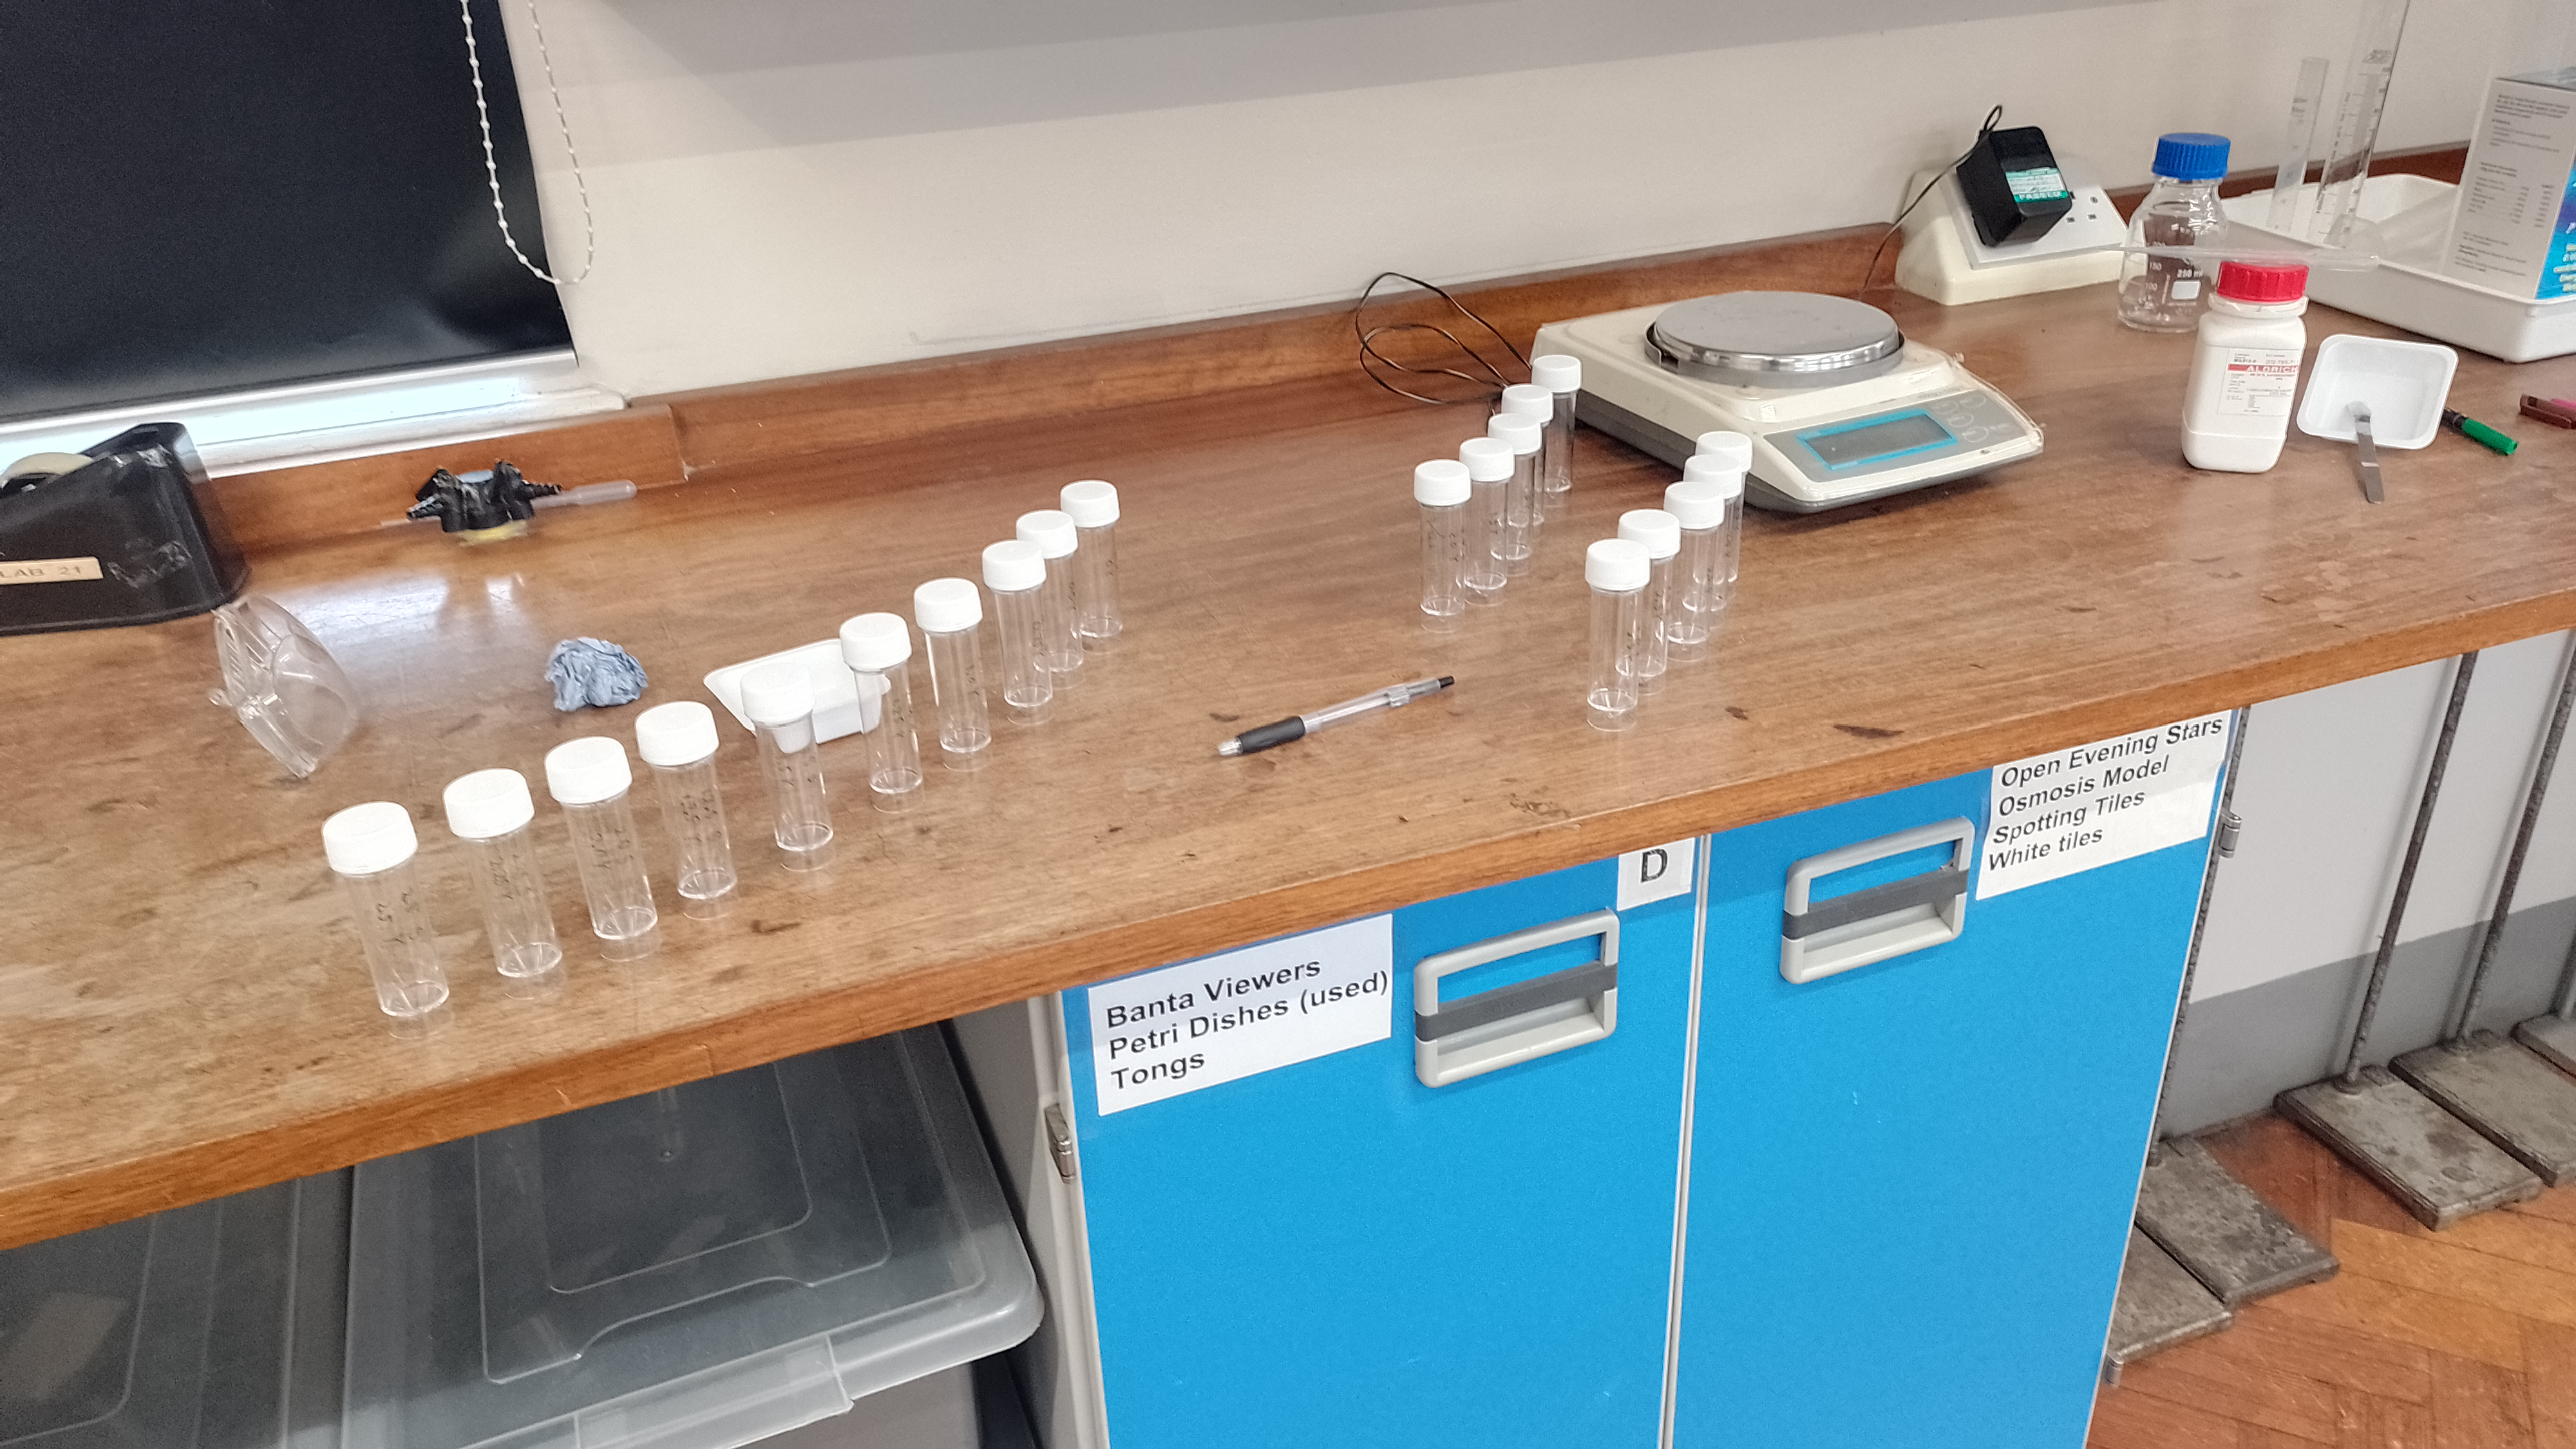
\includegraphics[width=0.45\textwidth]{vials-before}}
  \hfill
  \subfigure[Filled with slightly different media mix]{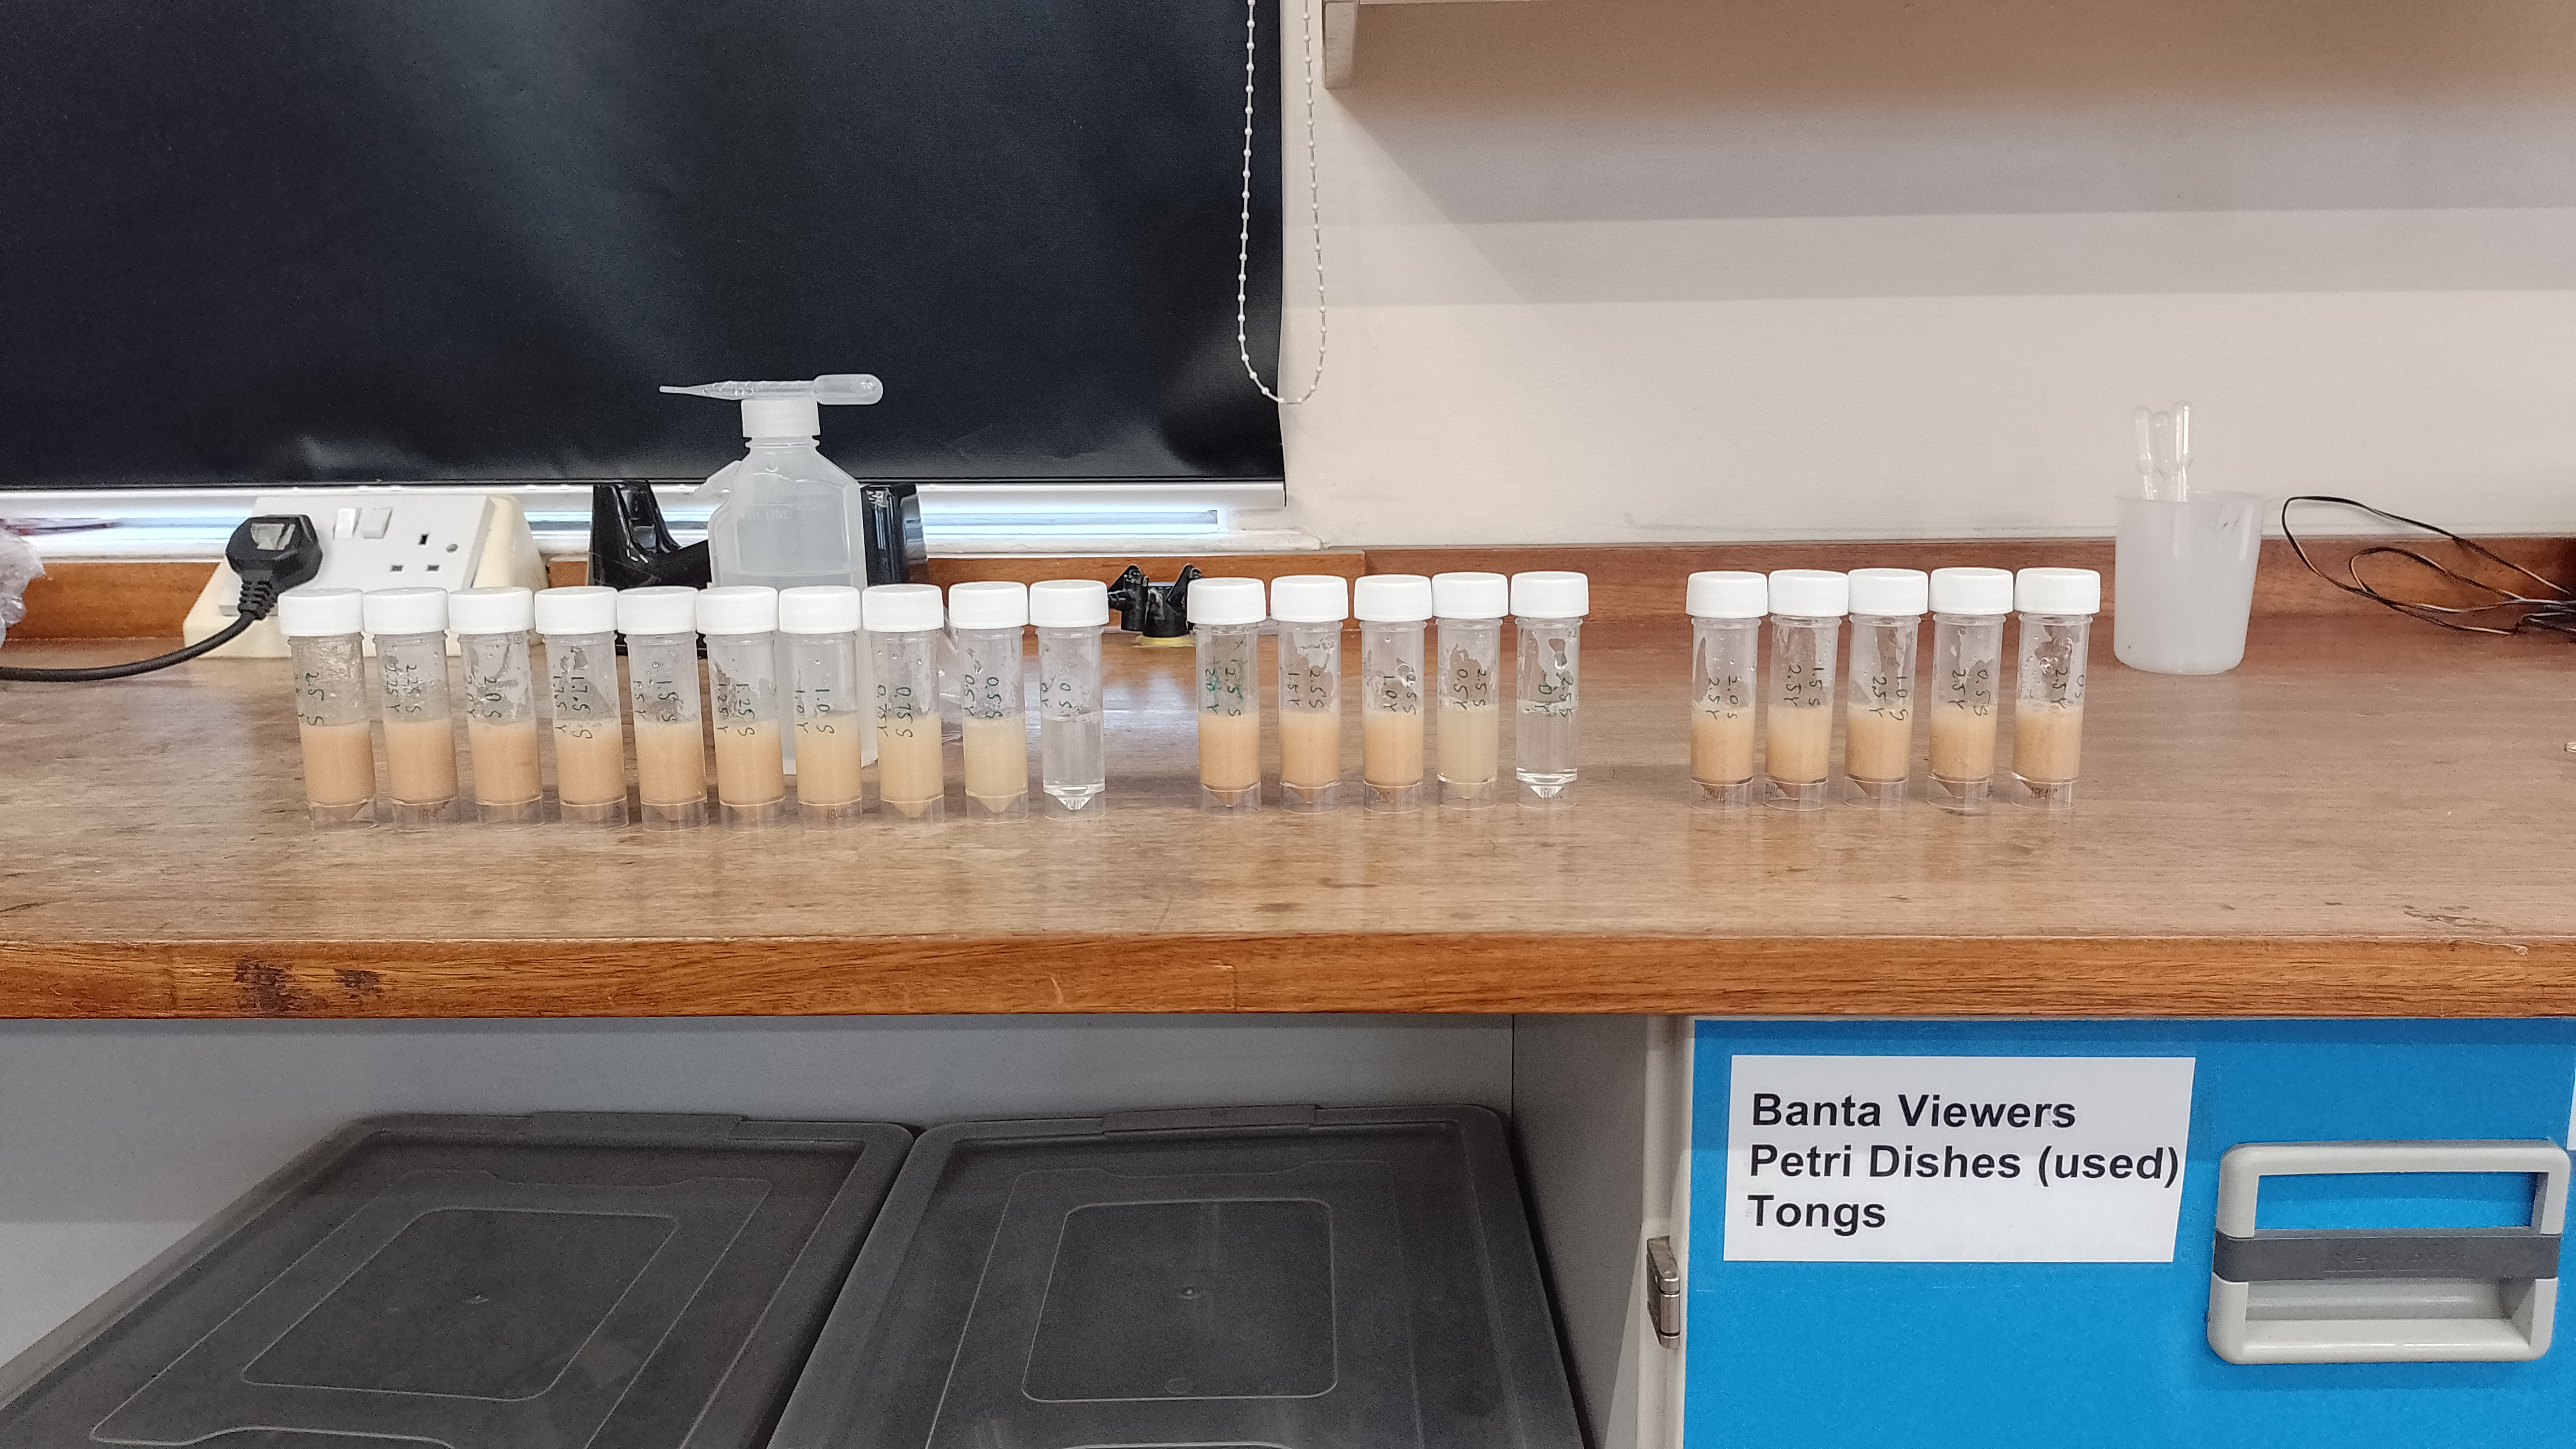
\includegraphics[width=0.45\textwidth]{vials-after}}
\end{figure}

\noindent\\
The rack of vials is then refrigerated to preserve it from moulds during the 2 weeks long Easter holidays.

\subsubsection{3rd May}

The flies arrived around 5 days ago, but because of the timings of weekends and strikes, the flies are starting to be put into vials only now.

\noindent\\
Last year the STEM biology class was shown how to transfer flies from one vial to another - use ice water to chill the vial, this put the flies to sleep. Now just tip the vials over the other and the flies will "pour" into the destination vial.

\noindent\\
This cannot be done to the big vials of flies here, because first of all, the vial is big. I don't think all the flies can be put to sleep using just ice water, so when I uncap the vial loads of still very active flies will just come out and make a big mess.

\noindent\\
For that I was provided FlyNap - a liquid which flies will go to sleep for a long period (around 10 minutes) after being exposed. It is used in enclosed spaces such as vials where the air doesn't circulate well, so the concentration of FlyNap can build up for the flies.

\noindent\\
I planned to sort the flies into male and female flies before putting them into vials. Which makes the whole process more systematic and *should* make it more efficient (it does not).

\noindent\\
Doing so allows me to know how many flies there are for each gender, and use division to find out how many flies of each gender to put into the vials. This is especially important as I am not sure that the ratio of male to female is going to be one-to-one.

\begin{enumerate}
  \item Use FlyNap to put the vial of flies into unconscious.
  \item Place 3 petri dishes in ice water - one for unsorted flies, one for males and the other for females.
  \item Pour a sizable number of flies from the large vial to the petri dishes of unsorted flies.
  \item Sort the flies into male and female.
  \item When all flies are sorted, count the total number of each gender and calculate the number of flies to put into each vial.
\end{enumerate}

\noindent
I originally thought a microscope will be needed to clearly identify the male and female flies, but in reality, their features can be identified by the naked eye. Neat.

\begin{figure}[ht]
  \centering
  \subfigure[The big vial of flies and the 20 vials i have to put them into]{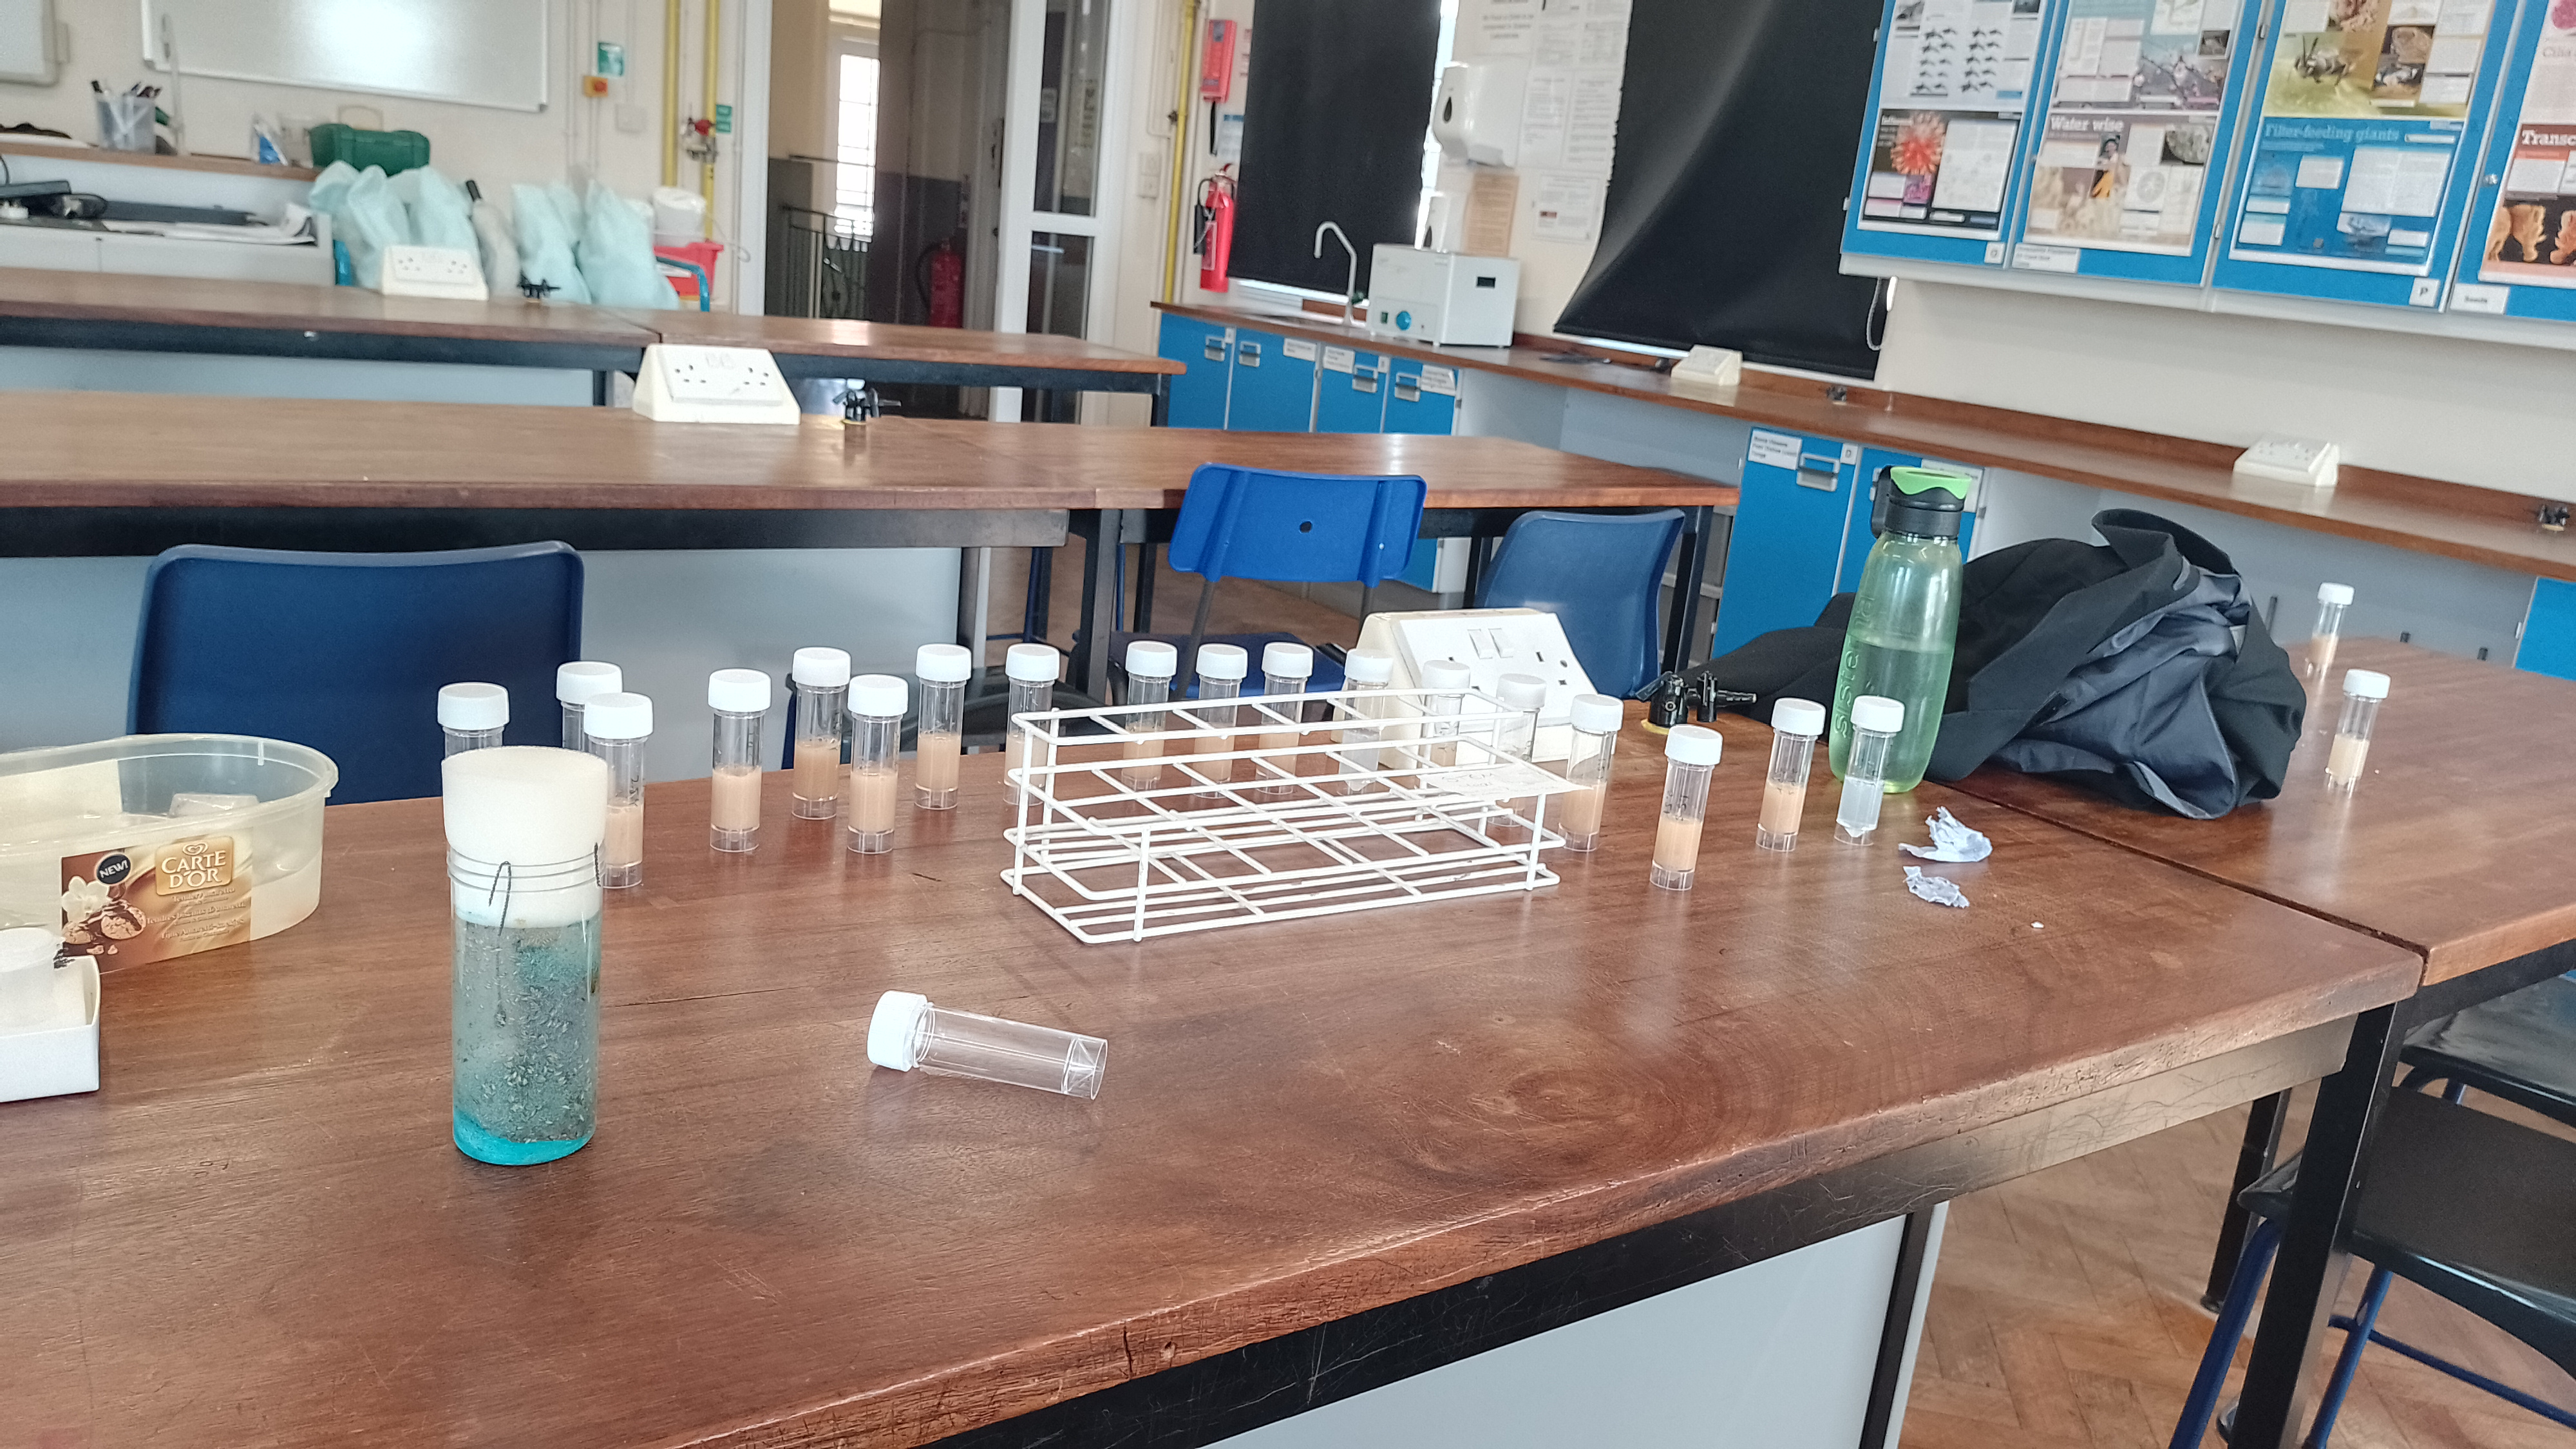
\includegraphics[height=0.25\textwidth]{to-vials}}
  \hfill
  \subfigure[Identifying male and female flies (online image)]{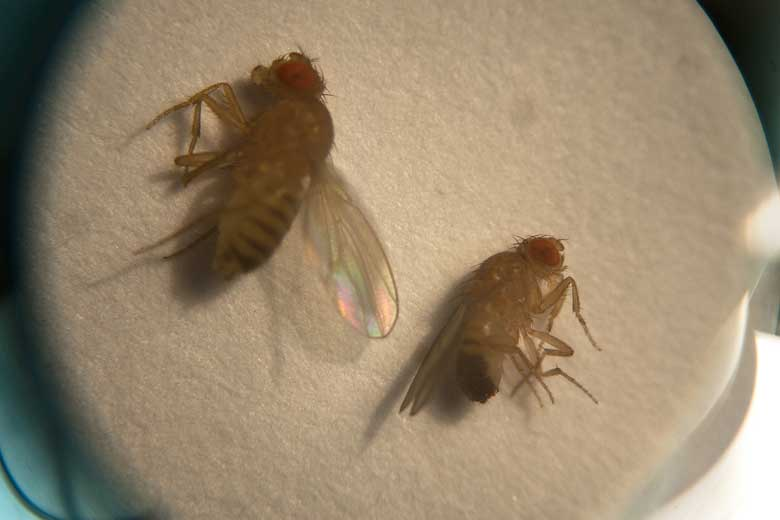
\includegraphics[height=0.25\textwidth]{fm-flies}}
\end{figure}

\noindent
What happened was a bit more of a mess, flies kept waking up and flying await even when chilled. Many of them jumped into the water and became inactive, I don't know if they are alive or not, but I continued to sort them anyways.

\noindent\\
This sorting effort continued to the day after, as conclusion 4 male and 5 female flies will be put into each vial. Then the vials are put into a rack and left for them to survive and reproduce.

\subsection{Recordings}

As mentioned, the recordings were taken with a note-taking app, in a plain text format.

\noindent\\
The vials of flies were put in the refrigerator until the 5th of May while I was sorting things out. And as of writing this, I've completely forgotten what was being sorted out, and the only thing I can be sure of is that the flies were refrigerated until Friday for some reason.

\noindent\\
Data may be inferred, for example, the number of active fruit flies for the first week is calculated by subtracting the number of inactive flies from the initial number of flies (9).

\newpage
\subsubsection{12th May (day 7)}

There seemed to be no reproduction yet, the media are all perfectly clean, and no larvae or pupa.\\

{
\centering
\begin{tabular}{|c|c|c|}
  \hline
  Sucrose & Yeast & Alive\\
  \hline
  \hline
  75 & 75 & 8\\
  67.5 & 67.5 & 8\\
  60 & 60 & 8\\
  52.5 & 52.5 & 9\\
  45 & 45 & 7\\
  37.5 & 37.5 & 9\\
  30 & 30 & 7\\
  22.5 & 22.5 & 9\\
  15 & 15 & 6\\
  0 & 0 & 2\\
  \hline
\end{tabular}
\begin{tabular}{|c|c|c|}
  \hline
  Sucrose & Yeast & Alive\\
  \hline
  \hline
  60 & 75 & 7\\
  45 & 75 & 8\\
  30 & 75 & 7\\
  15 & 75 & 9\\
  0 & 75 & 6\\
  \hline
  75 & 60 & 6\\
  75 & 45 & 9\\
  75 & 30 & 8\\
  75 & 15 & 8\\
  75 & 0 & 7\\
  \hline
\end{tabular}
\par
}

\subsubsection{19th May (day 14)}

Reproduction seemed to have started, and the new generations are currently at their pupa stage. This means most of the active fruit flies are still from the original 9.\\

{
\centering
\begin{tabular}{|c|c|c|c|c|c|}
  \hline
  Sucrose & Yeast & larvae & Pupa & Inactive & Active\\
  \hline
  \hline
  75 & 75 & 13 & 62 & least 5 & 8\\
  67.5 & 67.5 & 28 & 41 & - & 6\\
  60 & 60 & 26 & 47 & least 2 & 7\\
  52.5 & 52.5 & 20 & 76 & - & 7\\
  45 & 45 & 49 & 33 & 0 & 9\\
  37.5 & 37.5 & 32 & 19 & - & 6\\
  30 & 30 & 34 & 5 & 3 & 10\\
  22.5 & 22.5 & 30 & 0 & - & 8\\
  15 & 15 & 3 & 0 & 3 & 8\\
  0 & 0 & 0 & 0 & 9 & 0\\
  \hline
  60 & 75 & 21 & 48 & least 1 & 7\\
  45 & 75 & 40 & 5 & 2 & 7\\
  30 & 75 & 25 & 55 & least 2 & 7\\
  15 & 75 & 44 & 43 & - & 6\\
  0 & 75 & 40 & 68 & - & 0\\
  \hline
  75 & 60 & 8 & 27 & least 5 & 9\\
  75 & 45 & 14 & 24 & least 3 & 6\\
  75 & 30 & 12 & 52 & - & 6\\
  75 & 15 & 11 & 0 & 2 & 8\\
  75 & 0 & 0 & 0 & 2 & 7\\
  \hline
\end{tabular}
\par
}

\noindent\\
Here are a few other things noted down on certain vials:

\begin{itemize}
  \item 45/75 slight moulding.
  \item 75/15 larvae are digging deeper than usual (in comparison to other vials).
\end{itemize}
\newpage
\noindent
Most values starting from this recording will be estimations rather than accurate values. Reasons are:

\begin{itemize}
  \item larvae dig into the media mix, since the media mix is mostly opaque, I can only count the larvae that are very near the side of the vial, so the actual number may be much higher. (But this is still a fair recording as it is done to all vials)
  \item That problem is also true (to a lesser degree) for the pupa.
  \item Dead flies are impossible to count as they become a mash of goo mixed along with pupa and other materials.
\end{itemize}

\subsubsection{5th June (day 31)}

There was a big gap between the 2nd and the 3rd recording, this is because I couldn't do the recording on 26th May (the 21st day) when school is empty for some reason. Then there is a whole week of half-term holidays when school is closed.

\noindent\\
As you can see, I've given up recording the actual number of pupa and larvae. The flies have been making an absolute mess - the walls are getting dirty, and there are simply too many larvae and pupa to be counted. I therefore resort to a more subjective "does it have loads of X" recording to save me some time.

\noindent\\
I've also started recording how many mm of media mix the flies consumed, I figured out it would be useful to show if the flies consume around the same amount of nutrients (per fly) no matter the environment as a side investigation.\\

{
\centering
\begin{tabular}{|c|c|c|c|c|c|}
  \hline
  Sucrose & Yeast & Alive & Media eaten (mm) & Loads of larvae & Loads of pupa\\
  \hline
  \hline
  75 & 75 & 44 & 2 & true & true\\
  67.5 & 67.5 & 51 & 2 & true & true\\
  60 & 60 & 44 & 3 & true & true\\
  52.5 & 52.5 & 47 & 6 & true & true\\
  45 & 45 & 43 & 3 & true & false\\
  37.5 & 37.5 & 36 & 3 & false & false\\
  30 & 30 & 40 & 1 & false & false\\
  22.5 & 22.5 & 38 & 1 & false & false\\
  15 & 15 & 5 & 3 & false & false\\
  0 & 0 & 0 & 0 & false & false\\
  \hline
  60 & 75 & 47 & 4 & true & true\\
  45 & 75 & 16 & 3 & false & false\\
  30 & 75 & 28 & 4 & - & -\\
  15 & 75 & 11 & 6 & true & true\\
  0 & 75 & 13 & 4 & true & false\\
  \hline
  75 & 60 & 66 & 3 & true & false\\
  75 & 45 & 46 & 3 & false & true\\
  75 & 30 & 42 & 4 & false & true\\
  75 & 15 & 5 & 3 & false & false\\
  75 & 0 & 0 & 0 & false & false\\
  \hline
\end{tabular}
\par
}

\noindent\\
There wasn't a problem with vial 30/75, it's just that I forgot to record the two values.

\noindent\\
Here are some other things also noted down:

\begin{itemize}
  \item 45/75 appears to have very little pupa.
  \item More nutrients (the original note says "sucrose", but I guess I was biased) result in quicker movement and more active flies. For example, 75/75 is more active than 30/30.
\end{itemize}

\noindent
The media may have shrunk or be compared slightly for vials 0/0 and 75/0, but because of the way I measured how much the media mix has been consumed by comparing them to the 0/0 and 75/0 vials (which should not be consumed much), so by definition they have been consumed 0mm no matter what.

\noindent\\
This may make recordings less accurate, but one benefit of doing so is that it may unintentionally cancel out the shrinking of media mix in other vials, as a result of sunshine and water drying up.

\subsubsection{12th June (day 38)\\}

{
\centering
\begin{tabular}{|c|c|c|c|}
  \hline
  Sucrose & Yeast & Alive & Media eaten (mm)\\
  \hline
  \hline
  75 & 75 & 128 & 3\\
  67.5 & 67.5 & 94 & 3\\
  60 & 60 & 69 & 6\\
  52.5 & 52.5 & 74 & 9\\
  45 & 45 & 83 & 8\\
  37.5 & 37.5 & 65 & -\\
  30 & 30 & 54 & 2\\
  22.5 & 22.5 & 51 & 2\\
  15 & 15 & 21 & 3\\
  0 & 0 & 0 & 0\\
  \hline
  60 & 75 & 61 & 5\\
  45 & 75 & 57 & 2\\
  30 & 75 & 37 & 4\\
  15 & 75 & 20 & 6\\
  0 & 75 & 0 & 5\\
  \hline
  75 & 60 & 89 & 3\\
  75 & 45 & 63 & 5\\
  75 & 30 & 80 & 3\\
  75 & 15 & 4 & 2\\
  75 & 0 & 0 & 0\\
  \hline
\end{tabular}
\par
}

\newpage
\noindent
Other details noted down:

\begin{itemize}
  \item 52.5/52.5 Many are dead.
  \item 0/75 moulding.
  \item 75/60 Some escaped because of my bad taping.
  \item 75/15 Their movement is slow.
\end{itemize}

\subsubsection{19th June (day 45) final recording}

So many of the vials have dried out so as of this recording, making many of the vials invalid as the flies are dying because of external reasons.\\

{
\centering
\begin{tabular}{|c|c|c|c|c|}
  \hline
  Sucrose & Yeast & Alive & Media eaten (mm) & Dried out\\
  \hline
  \hline
  75 & 75 & 44 & 4 & false\\
  67.5 & 67.5 & 14 & 4 & false\\
  60 & 60 & 2 & 5 & true\\
  52.5 & 52.5 & 3 & 7 & true\\
  45 & 45 & 2 & 6 & true\\
  37.5 & 37.5 & 3 & 5 & true\\
  30 & 30 & 39 & 2 & false\\
  22.5 & 22.5 & 26 & 2 & false\\
  15 & 15 & 12 & 4 & false\\
  0 & 0 & 0 & 0 & false\\
  \hline
  75 & 60 & 75 & 3 & false\\
  75 & 45 & 80 & 3 & false\\
  75 & 30 & 74 & 4 & false\\
  75 & 15 & 3 & 3 & false\\
  75 & 0 & 0 & 0 & false\\
  \hline
  60 & 75 & 4 & 7 & true\\
  45 & 75 & 68 & 2 & false\\
  30 & 75 & 1 & 2 & true\\
  15 & 75 & 0 & 4 & false\\
  0 & 75 & 0 & 3 & false\\
  \hline
\end{tabular}
\par
}

\subsection{Disposal}

The flies are native species, and I was told to just let them go.

\begin{figure}[ht]
  \centering
  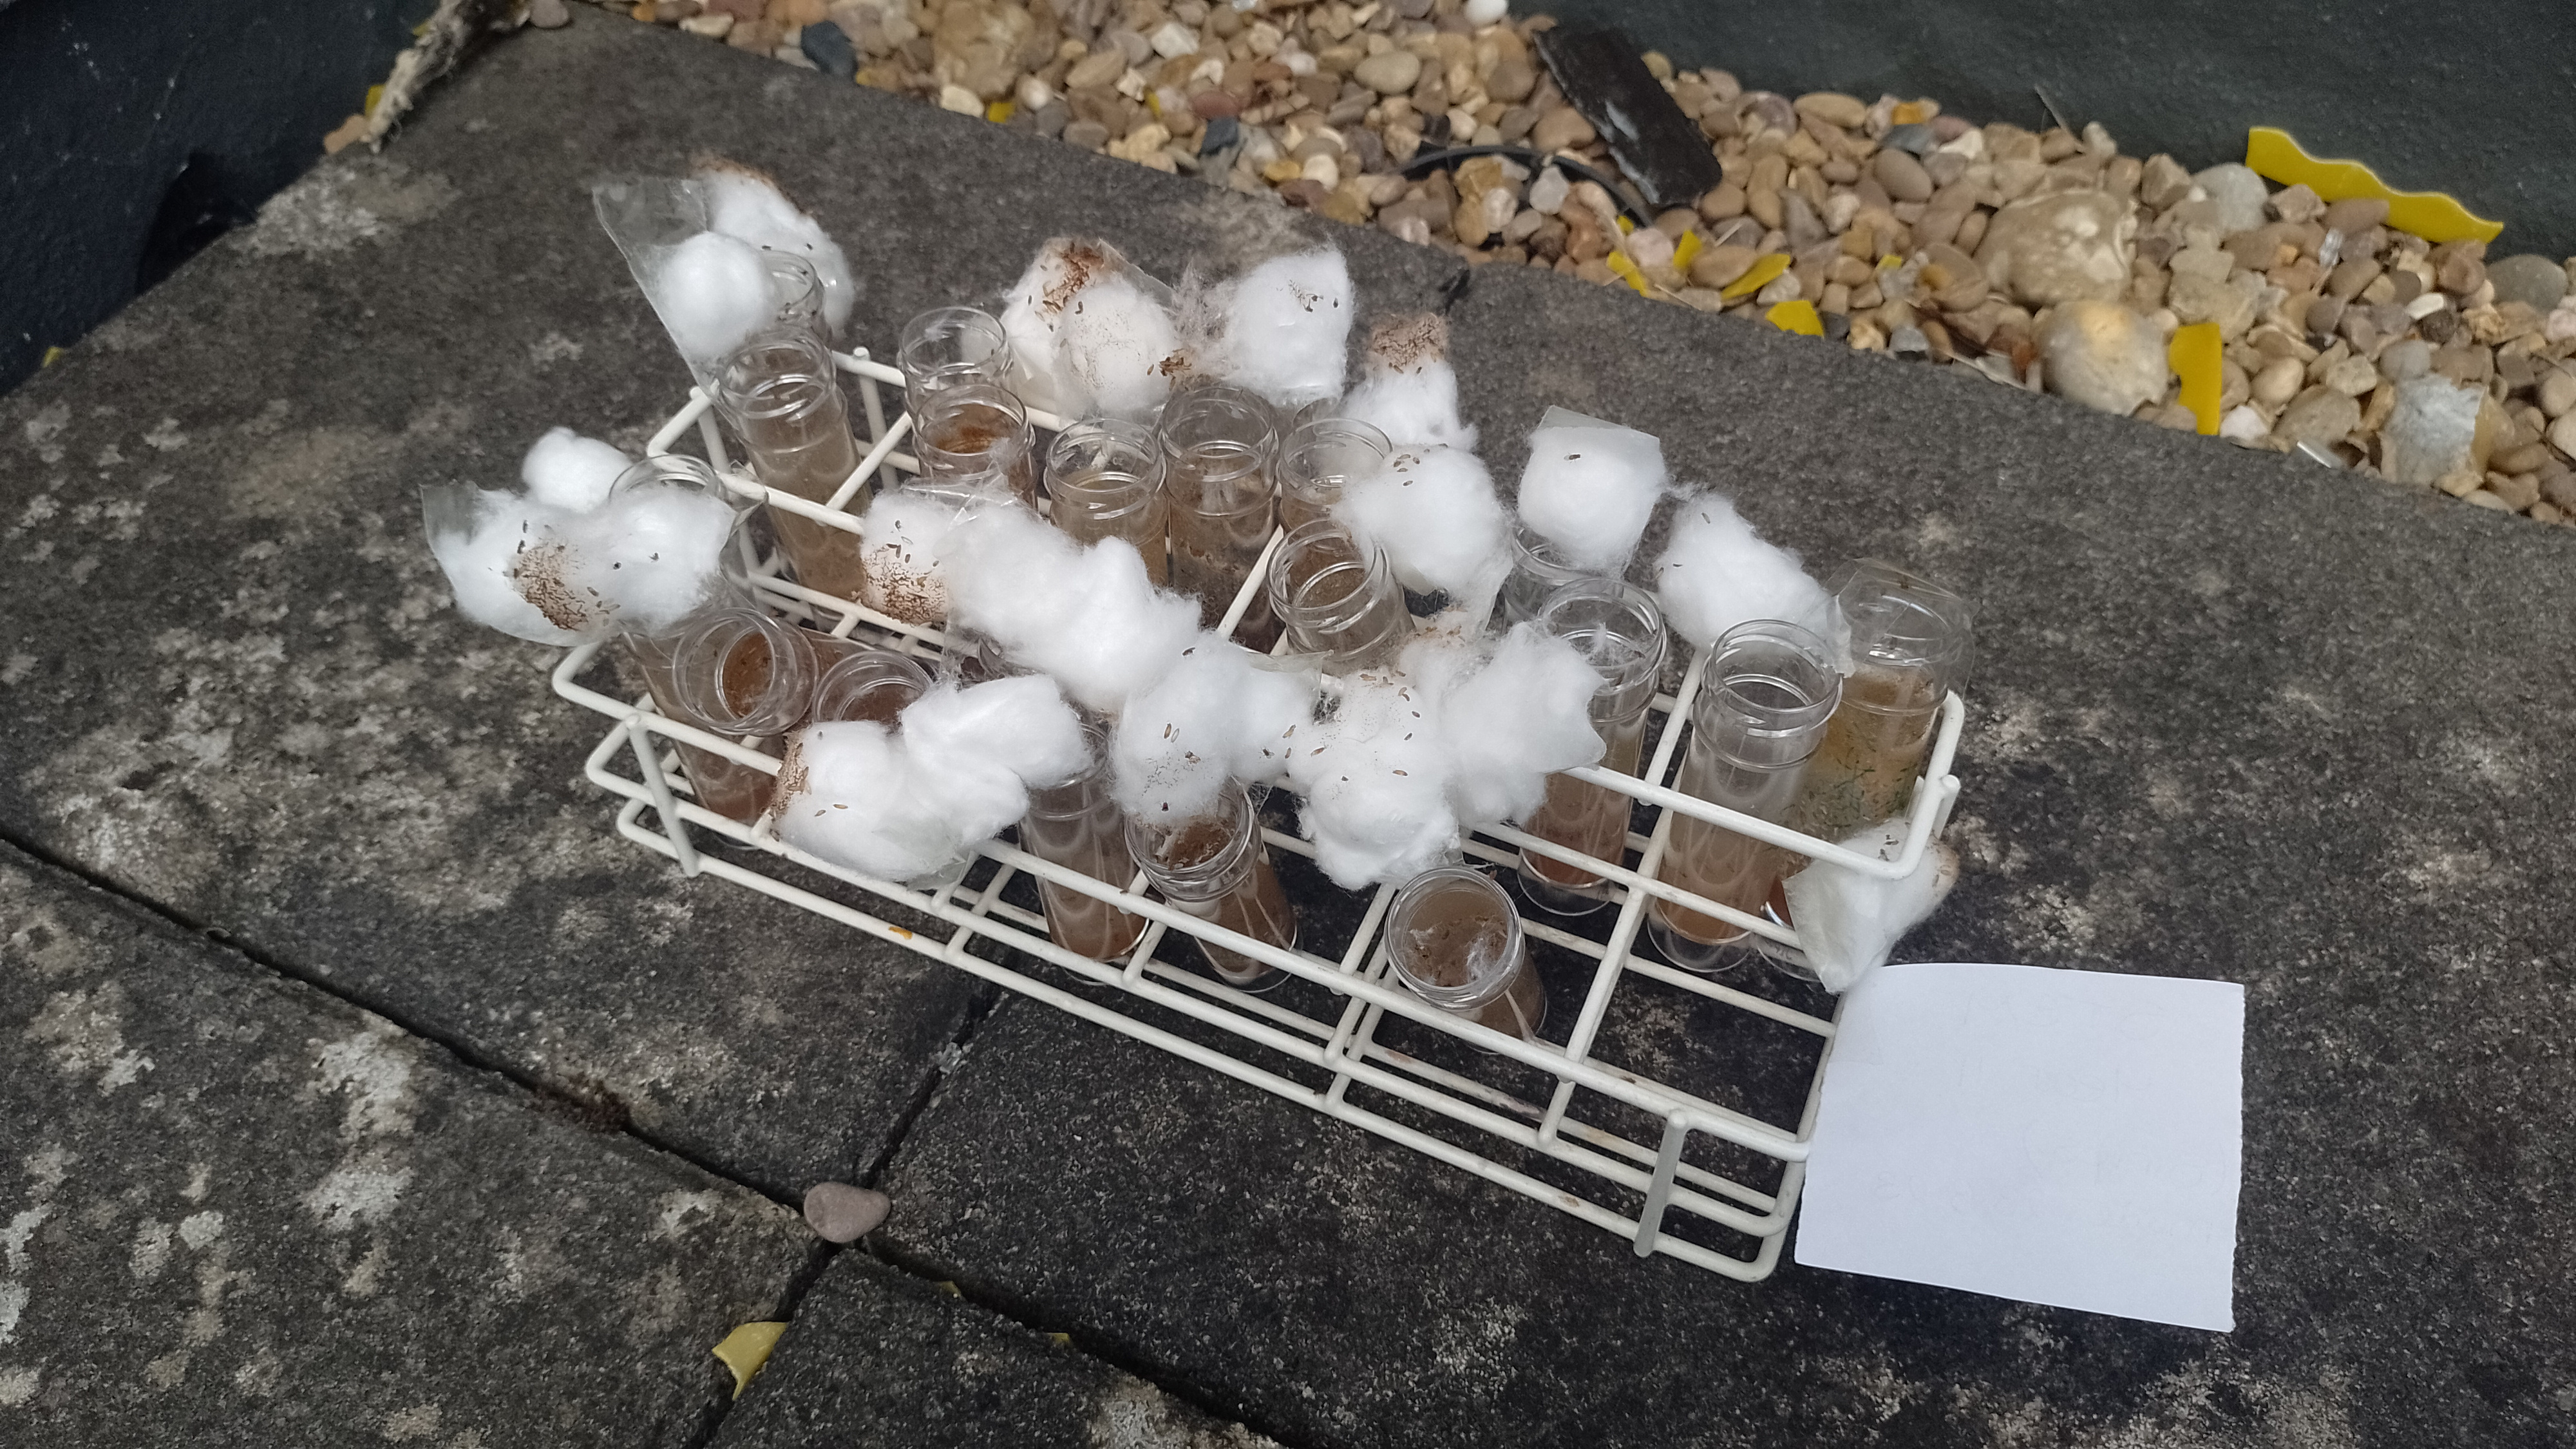
\includegraphics[width=120px]{letemgo}
\end{figure}

\section{Evalutation}

Lines of best fit from www.omnicalculator.com/statistics/polynomial-regression

\subsection{Finding point of malnourishment}

Although this is not one of the hypotheses, I did think there should be a "point of malnourishment" which can be used to separate "sufficient" nutrients to the left, and "insufficient" nutrients to the right.

\noindent\\
Plotting the data to the graph with a line of best fit:

\begin{center}
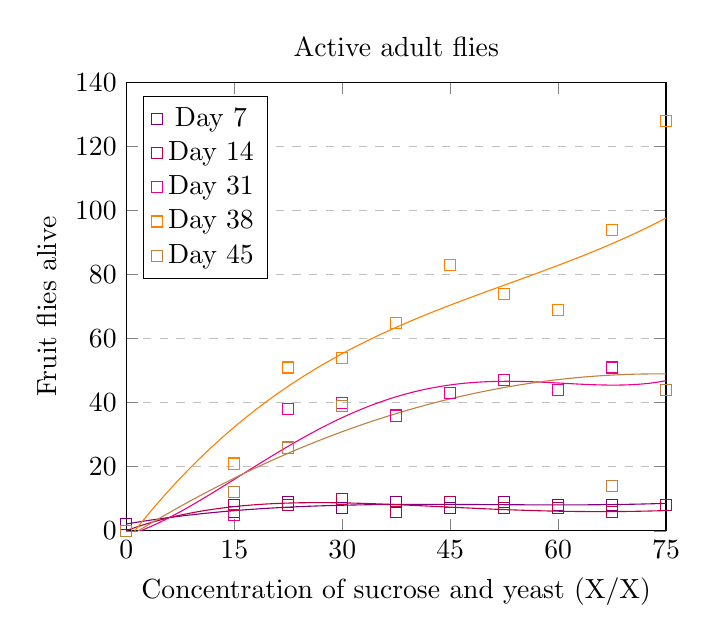
\begin{tikzpicture}
  \begin{axis}[
    title={Active adult flies},
    xlabel={Concentration of sucrose and yeast (X/X)},
    ylabel={Fruit flies alive},
    xmin=0, xmax=75,
    ymin=0, ymax=140,
    xtick={0,15,30,45,60,75},
    ytick={0,20,40,60,80,100,120, 140},
    legend pos=north west,
    ymajorgrids=true,
    grid style=dashed,
]

  \addplot[
    only marks,
    color=violet,
    mark=square,
  ]
  coordinates{
    (0,2)(15,6)(22.5,9)(30,7)(37.5,9)(45,7)(52.5,9)(60,8)(67.5,8)(75,8)
  };
  \addlegendentry{Day 7}
    
  \addplot[
    only marks,
    color=purple,
    mark=square,
  ]
  coordinates {
    (0,0)(15,8)(22.5,8)(30,10)(37.5,6)(45,9)(52.5,7)(60,7)(67.5,6)(75,8)
  };
  \addlegendentry{Day 14}
  

  \addplot[
    only marks,
    color=magenta,
    mark=square,
  ]
  coordinates {
    (0,0)(15,5)(22.5,38)(30,40)(37.5,36)(45,43)(52.5,47)(60,44)(67.5,51)(75,44)
  };
  \addlegendentry{Day 31}

  \addplot[
    only marks,
    color=orange,
    mark=square,
  ]
  coordinates {
    (0,0)(15,21)(22.5,51)(30,54)(37.5,65)(45,83)(52.5,74)(60,69)(67.5,94)(75,128)
  };
  \addlegendentry{Day 38}

  \addplot[
    only marks,
    color=brown,
    mark=square,
  ]
  coordinates {
    (0,0)(15,12)(22.5,26)(30,39)(67.5,14)(75,44)
  };
  \addlegendentry{Day 45}

  \addplot [
    domain=0:75, 
    samples=100, 
    color=violet,
    ]
    {0.000051*x^3-0.00778*x^2+0.382514*x+2.136369};
  \addplot [
    domain=0:75, 
    samples=100, 
    color=purple,
    ]
    {-0.000001*x^4+0.000278*x^3-0.024972*x^2+0.814395*x+0.075425};
  \addplot [
    domain=0:75, 
    samples=100, 
    color=magenta,
    ]
    {0.0000084*x^4-0.001285*x^3+0.048214*x^2+0.714434*x-1.578422};
  \addplot [
    domain=0:75, 
    samples=100, 
    color=orange,
    ]
    {0.00025*x^3-0.039775*x^2+2.923647*x-3.334842};
  \addplot [
    domain=0:75, 
    samples=100, 
    color=brown,
    ]
    {-0.009425*x^2+1.39034*x-2.272553};
  \end{axis}
\end{tikzpicture}
\end{center}

\noindent
(Graph above shows data only for X/X vials, such as 75/75 and 0/0)

\noindent\\
What we can look for is an inflection point on the graph, that should be the point separating mal and non-malnourishment. This is because the rate of increase in active flies should be different depending on whether there are already enough nutrients - the rate of increase when there are already sufficient nutrients should be slower since the number of fruit flies is already closer to saturation. Resulting in a gentler slope.

\noindent\\
Looking at the graph, the inflection point seemed to differ from recording to recording, but generally between 25 and 50. The range is relatively large, but the inflection point is there.

\noindent\\
Knowing this could be helpful, as the slope plateaus to the right of this point. Making random errors seem more significant, it's just good to know that data beyond this point will be much noisier and perhaps less reliable to compare against each other (as their differences may be caused by noise).

\noindent\\
We can also see that the data from the beginning of the experiment (especially the first week) doesn't seem very important.

\subsection{The first hypothesis}

\subsubsection{Analysing recording data for hypothesis 1}

The first hypothesis is all about reproduction to survival rate ratio, which as mentioned can be calculated using

$$\text{reproduction-survival ratio}=\frac{(\text{no. of larvae}+\text{pupa})^2}{\text{initial no.}\times\text{adult flies}}$$

\begin{table}[h]
\centering
\begin{tabular}{|c|c|c|c|}
  \hline
  Concentration & larvae + pupa & Ratio (day 31) & Ratio (day 38)\\
  \hline
  \hline
  0 & 0 & 0 & 0\\
  15 & 3 & 0.2 & 0.0476\\
  22.5 & 30 & 2.6316 & 1.9608\\
  30 & 39 & 4.225 & 3.1296\\
  37.5 & 51 & 8.0278 & 4.4462\\
  45 & 82 & 17.3747 & 9.0013\\
  52.5 & 96 & 21.7872 & 13.8378\\
  60 & 73 & 13.4571 & 8.5813\\
  67.5 & 69 & 10.3725 & 5.6277\\
  75 & 75 & 14.2045 & 4.8828\\
  \hline
\end{tabular}
\end{table}

\noindent\\
If the hypothesis is correct, then the reproduction-to-survival ratio should be higher when there are fewer nutrients. However, this certainly does not seem to be the case here, as the ratio increases with the abundance of nutrients.

\noindent\\
Now plotting it into a graph:

\begin{center}
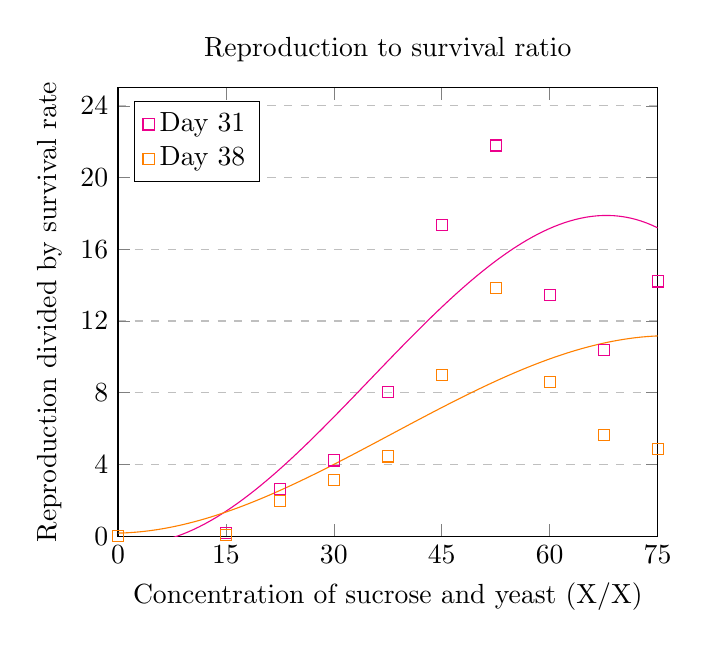
\begin{tikzpicture}
  \begin{axis}[
    title={Reproduction to survival ratio},
    xlabel={Concentration of sucrose and yeast (X/X)},
    ylabel={Reproduction divided by survival rate},
    xmin=0, xmax=75,
    ymin=0, ymax=25,
    xtick={0,15,30,45,60,75},
    ytick={0,4,8,12,16,20,24},
    legend pos=north west,
    ymajorgrids=true,
    grid style=dashed,
]

  \addplot[
    only marks,
    color=magenta,
    mark=square,
  ]
  coordinates {
    (0,0)(15,0.2)(22.5,2.6316)(30,4.225)(37.5,8.0278)(45,17.3747)(52.5,21.7872)(60,13.4571)(67.5,10.3725)(75,14.2045)
  };
  \addlegendentry{Day 31}

  \addplot[
    only marks,
    color=orange,
    mark=square,
  ]
  coordinates {
    (0,0)(15,0.0476)(22.5,1.9608)(30,3.1296)(37.5,4.4462)(45,9.0013)(52.5,13.8378)(60,8.5813)(67.5,5.6277)(75,4.8828)
  };
  \addlegendentry{Day 38}

  \addplot [
    domain=0:75, 
    samples=100, 
    color=magenta,
    ]
    {-0.000129*x^3+0.013548*x^2-0.056093*x-0.384073};
  \addplot [
    domain=0:75, 
    samples=100, 
    color=orange,
    ]
    {-0.000048*x^3+0.005462*x^2+0.006931*x+0.173645};
  \end{axis}
\end{tikzpicture}
\end{center}

\newpage
\subsubsection{Evaluating hypothesis 1}
Since we know that the data above 50 is just noise, it can be simply ignored.

\noindent\\
Ignoring any points above 50, we can see that the results match perfectly\dots\space to the opposite of what the hypothesis predicts.

\noindent\\
I thought this couldn't be right, but the maths makes sense. After searching around for a while, I thought it would be the number of larvae which might be causing issues, as only the larvae around the walls of the vials are counted - there may be much more not counted. As an attempt to cancel this error, I tried multiplying the number of larvae by a factor of 8, but it still gave me a similar result.

\subsubsection{Conclusions on hypothesis 1}
Not only was the hypothesis not supported, it seems like the opposite is true.

\noindent\\
The experiment shows that as the abundance of nutrients drops, the fruit flies tend to stop reproducing first and save that resources for survival. This makes for a way less interesting hypothesis than the flies prioritising reproduction before survival, but I guess it makes sense that reproduction comes after basic survival needs.

\subsection{The second hypothesis}

The easiest way to support the second hypothesis would be to compare similar vials from the two series (X/75 and 75/X).

\subsubsection{Comparing vials}

One of the more useful comparisons is between the vials 75/0 and 0/75 at day 14.\\

{
\centering
\begin{tabular}{|c|c|c|c|c|c|}
  \hline
  Sucrose & Yeast & larvae & Pupa & Inactive & Active\\
  \hline
  \hline
  0 & 75 & 40 & 68 & - & 0\\
  75 & 0 & 0 & 0 & 2 & 7\\
  \hline
\end{tabular}
\par
}

\noindent\\
They show the two extremes from the two series of vials, to sum up the differences:

\begin{itemize}
  \item Vial with no sucrose has no flies alive, while the vial with sucrose still has most of the flies active, showing that sucrose (glucose) is responsible for the survival of the flies.
  \item Vial with no yeast has no reproduction at all, while the vials with yeast has a large number of reproduction, showing that yeast (protein) is crucial for the reproduction of the flies.
\end{itemize}

\noindent
The comparison supports the 2nd hypothesis, as it showed that each glucose and protein has distinct and irreplaceable roles for the survival and reproduction of the flies. However, many flies from the 0/75 vial (yeast only) successfully grew from larvae into pupa, and adult flies, this may suggest that glucose is not that crucial to the flies' survival, which can be a result of protein also able to provide a source of energy. The fact that yeast of the same concentration is a lot less energy dense than sucrose, can explain why there are no active flies in the 0/75 vial at day 14.

\subsubsection{Analysing recording data for hypothesis 2}

To support hypothesis 2, the recording data must show the survival rate dropping quicker than the reproduction rate as the amount of sucrose decreases, and the reproduction rate dropping quicker than the survival rate as the amount of yeast decreases.

\begin{table}[h]
\centering
\begin{tabular}{|c|c|c|c|c|c|c|}
  \hline
  Sucrose & Yeast & larvae + pupa & Active (day 31) & Ratio (day 31) & Active (day 38) & Ratio (day 38)\\
  \hline
  \hline
  75 & 75 & 75 & 44 & 14.2045 & 128 & 4.8828\\
  \hline
  60 & 75 & 69 & 47 & 11.2553 & 61 & 8.6721\\
  45 & 75 & 45 & 16 & 14.0625 & 57 & 3.9474\\
  30 & 75 & 80 & 28 & 25.3968 & 37 & 19.2192\\
  15 & 75 & 87 & 11 & 76.4545 & 20 & 42.05\\
  0 & 75 & 108 & 13 & 99.6923 & 0 & 0\\
  \hline
  75 & 60 & 35 & 66 & 2.0623 & 89 & 1.5293\\
  75 & 45 & 38 & 46 & 3.4879 & 63 & 2.5467\\
  75 & 30 & 64 & 42 & 10.8360 & 80 & 5.6889\\
  75 & 15 & 11 & 5 & 2.6889 & 4 & 3.3611\\
  75 & 0 & 0 & 0 & 0 & 0 & 0\\
  \hline
\end{tabular}
\end{table}

\noindent
Looking at the numbers, it matches the hypothesis. As the amount of sucrose decreases, the reproduction to survival ratio increases, because $\frac{\text{reproduction rate}}{\text{survival rate}}$: as survival rate decreases with the concentration of sucrose, and reproduction rate stays largely the same (from an unvarying amount of yeast), the number skyrockets as the concentration of sucrose gets close to 0.

\noindent\\
The reducing-yeast side also supports the hypothesis, as sucrose stays the same, the survival rate also stays largely the same, while the reproduction rate decreases with the amount of yeast. Therefore the ratio is lower when the yeast concentration is closer to 0.


\begin{center}
\begin{minipage}{.45\linewidth}
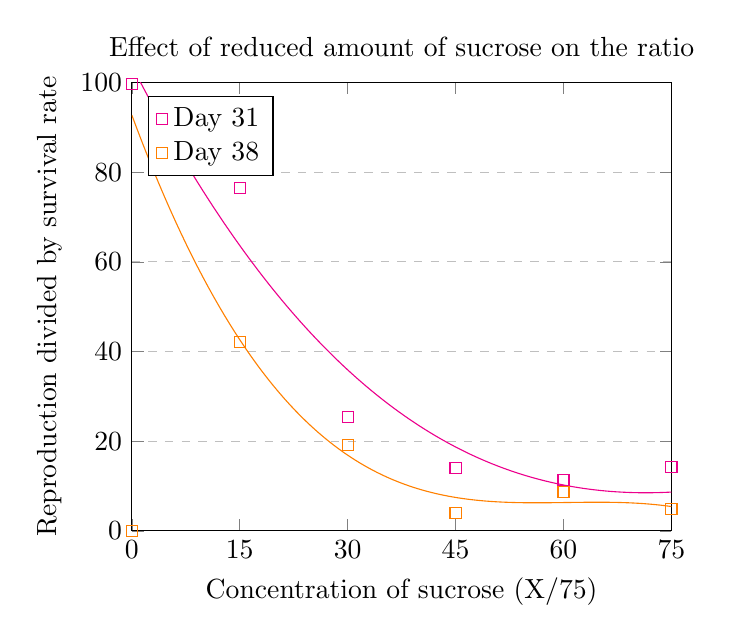
\begin{tikzpicture}
  \begin{axis}[
    title={Effect of reduced amount of sucrose on the ratio},
    xlabel={Concentration of sucrose (X/75)},
    ylabel={Reproduction divided by survival rate},
    xmin=0, xmax=75,
    ymin=0, ymax=100,
    xtick={0,15,30,45,60,75},
    ytick={0,20,40,60,80,100},
    legend pos=north west,
    ymajorgrids=true,
    grid style=dashed,
]

  \addplot[
    only marks,
    color=magenta,
    mark=square,
  ]
  coordinates {
    (0,99.6923)(15,76.4545)(30,25.3968)(45,14.0625)(60,11.2553)(75,14.2045)
  };
  \addlegendentry{Day 31}

  \addplot[
    only marks,
    color=orange,
    mark=square,
  ]
  coordinates {
    (0,0)(15,42.05)(30,19.2192)(45,3.9474)(60,8.6721)(75,4.8828)
  };
  \addlegendentry{Day 38}

  \addplot [
    domain=0:75, 
    samples=100, 
    color=magenta,
    ]
    {-0.00009*x^3+0.03153*x^2-3.126809*x+103.763771};
  \addplot [
    domain=0:75, 
    samples=100, 
    color=orange,
    ]
    {-0.000397*x^3+0.072015*x^2-4.33264*x+92.7607};
  \end{axis}
\end{tikzpicture}
\end{minipage}
\hfill
\begin{minipage}{.45\linewidth}
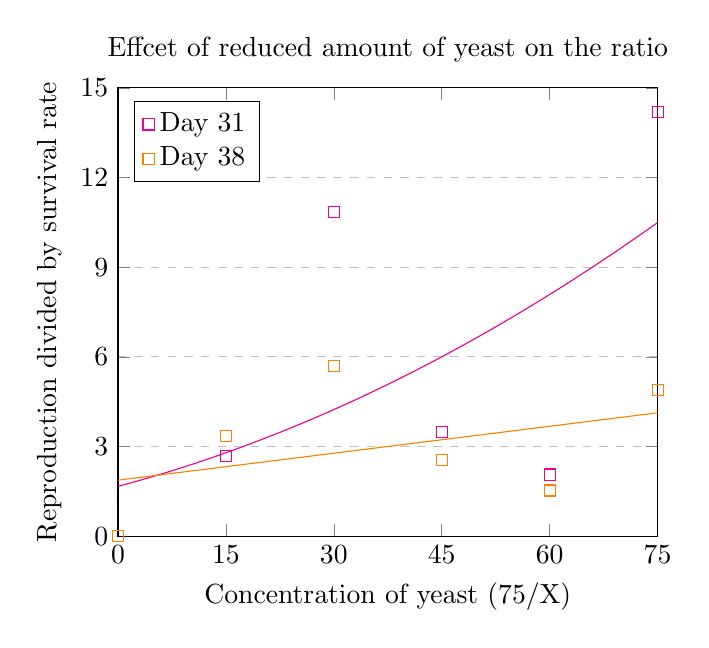
\begin{tikzpicture}
  \begin{axis}[
    title={Effcet of reduced amount of yeast on the ratio},
    xlabel={Concentration of yeast (75/X)},
    ylabel={Reproduction divided by survival rate},
    xmin=0, xmax=75,
    ymin=0, ymax=15,
    xtick={0,15,30,45,60,75},
    ytick={0,3,6,9,12,15},
    legend pos=north west,
    ymajorgrids=true,
    grid style=dashed,
]

  \addplot[
    only marks,
    color=magenta,
    mark=square,
  ]
  coordinates {
    (0,0)(15,2.6889)(30,10.8360)(45,3.4879)(60,2.0623)(75,14.2045)
  };
  \addlegendentry{Day 31}

  \addplot[
    only marks,
    color=orange,
    mark=square,
  ]
  coordinates {
    (0,0)(15,3.3611)(30,5.6889)(45,2.5467)(60,1.5293)(75,4.8828)
  };
  \addlegendentry{Day 38}

  \addplot [
    domain=0:75, 
    samples=100, 
    color=magenta,
    ]
    {0.000712*x^2+0.064277*x+1.666968};
  \addplot [
    domain=0:75, 
    samples=100, 
    color=orange,
    ]
    {0.03005*x+1.874581};
  \end{axis}
\end{tikzpicture}
\end{minipage}
\end{center}

\subsubsection{Conclusions for hypothesis 2}

The recording data shows support for hypothesis 2 - no modifications are needed for the hypothesis.

\section{Wrapping it all up}

To wrap it all up, a total of 2 hypotheses were tested by experiment. One passed the other one failed, the cool part is that seemingly random numbers from recordings could be organised in a way, where it is possible to use them to make solid claims about whether a hypothesis stands.

\noindent\\
I started doing the experiment believing "I just record everything, and figure out what to do with the data afterward". This is highly unideal as I have no idea what to do with the numbers: or how to use them to support the hypotheses until midway through writing this report.

\subsection{Improvements}

First of all, if I'm doing similar investigations again, I would set up the experiment in a way that I know can support the hypothesis with it. Making so the data can support the hypothesis is part of the planning, and should not be only thought of after the experiment, or else the effort may go to waste.

\noindent\\
Second of all, I don't need that much data - some recordings can be skipped. For example, the only few bits of data I needed were:

\begin{itemize}
  \item Alive flies on days 31 and 38.
  \item larvae and pupa count at day 14.
\end{itemize}

\noindent
This can be prevented, by again, planning the experiment before doing so. So that you will know what data you need and what recordings you don't need to make. I can say I spend a total of around 4 hours just counting flies and making recordings, and this can be cut in half if I've done any planning on what to record and what not to.

\noindent\\
I've also collected some useless data such as using true or false to represent "loads of larvae" and "loads of pupa" (day 31), those were completely useless, and I should've known that they will not be useful at all.

\noindent\\
I've also tried to start a "side investigation" to see how much nutrients a single fly consumes, and does a changing environment affects how much nutrients they consume (e.g. higher sucrose concentration$\to$more movement$\to$more sucrose consumption).

\noindent\\
This is a bad idea because when you already have 2 hypotheses waiting, you will not want to do another one. This is exactly what happened - it doesn't seem to be a very interesting investigation, so I just recorded the needed data and never made a conclusion on it.

\noindent\\
The better practice should be, to make an investigation plan and stick to it, with no side investigations, and no unneeded recordings.

\subsubsection{Suggestions}

To anyone who is doing fruit flies related experiments, here are some suggestions.

\begin{itemize}
  \item Use FlyNap, ice water just wouldn't work and makes a mess.
  \item Don't just sort them by gender and store them in petri dish, they get stuck in the dish, and there are so many flies in the big vial you'll never run out anyways.
  \item Seal it with extra cotton, if your vial is sealed with just enough cotton, that's not enough.
  \item Also if it wasn't already obvious, cotton allows the gas exchange of the flies, don't just cap the air off.
  \item Avoid sunlight at all costs, they cut your experiment short when the media mix dries out.
  \item 10ml of media mix maybe can last you around 40 days, so depending on how long you need your experiment to be, use a bigger vial and prepare more media mix per vial.
\end{itemize}

\noindent
Then there are some general suggestions about carrying out a general investigation.

\begin{itemize}
  \item Make a plan, record only what you need (and maybe a bit more).
  \item Don't record it in a format you know it's not useful, a more simple way of saying that is to only record numbers.
  \item Scatter diagrams are just amazing, use them always. And use a polynomial regression calculator to figure out a line of best fit.
  \item Write your report with \LaTeX\space instead of word or anything else, see how cool this is.
\end{itemize}

\subsection{Ending notes}

I joked about writing a 20-page report on this, I actually did it. Great job.

\noindent\\
No AI tools were used to write the paragraphs (except for help in \LaTeX\space syntax because I don't know how to), I also did threw the entire thing into Grammarly for spellcheck. I've alse used spreadsheets for doing some of the calculations (I've not used spreadsheet for so long).

\noindent\\
All the \LaTeX\space source files and other info are available on https://siriusmart.github.io/crest2023
\end{document}